\documentclass[10pt, a4paper]{report}
\usepackage{fontspec}            % Must use XeLaTeX
\setmainfont{Times New Roman}    % Or "DejaVu Serif", "Libertinus Serif"
% \setlength{\parskip}{15pt}
\usepackage{fancyhdr}
\usepackage{tikzlings}
\usepackage{sectsty} % For coloring section headings
\usepackage{pdfpages}
\usepackage{minitoc}
\usepackage{epstopdf}
\usepackage{graphicx}
\usepackage{fontawesome}
\usepackage{pifont}
\usepackage{booktabs}
\usepackage[
backend=biber,
style=numeric,
sorting=none
]{biblatex}

\addbibresource{references.bib}
\usepackage{placeins}
\setlength{\parskip}{10pt} % Adjust the amount of space here
\usepackage{float}
\usepackage{multirow}
\usepackage{tabularx}
\usepackage{adjustbox}
\usepackage{listings}
\usepackage{xcolor} % For coloring the code
\usepackage{algorithm}
\usepackage[noend]{algpseudocode}
\usepackage{siunitx}
\usepackage{subcaption}
\usepackage{indentfirst}
\setlength{\parindent}{1cm}
\setlength{\parskip}{0pt}
\usepackage[most]{tcolorbox}
\usepackage{enumerate}
\usepackage{tikz,tkz-tab}
\tikzset{set/.style={draw,circle,inner sep=0pt,align=center}}
\usepackage{parcolumns}
\usetikzlibrary{shapes.geometric}
\usepackage{wasysym}
\usepackage{enumitem}
\usepackage{ragged2e}
\usepackage{etoolbox}

\usepackage[tikz]{bclogo}
\usepackage{longfbox}
\usepackage{pgfplots}
\usepackage{footnote}
\usepackage[vietnamese]{babel}
\usepackage[colorlinks=true, linkcolor=black, citecolor=black, urlcolor=blue]{hyperref}
\usepackage{setspace}
% \doublespacing
\usetikzlibrary {positioning,graphs,calc,decorations.pathmorphing,shapes,arrows.meta,arrows,shapes.misc,fit,patterns}
\usepgfplotslibrary{fillbetween}
\pgfplotsset{compat=1.9}
\usepackage[explicit]{titlesec}
\usepackage{lipsum}

% Define your colors
\definecolor{titlebgdark}{RGB}{0,163,243}
\definecolor{chapnumberbg}{RGB}{1,84,164}
\definecolor{chapname}{RGB}{1,84,164}

\rhead{\faBook \color{gray}\textbf{ \leftmark}}
\lhead{\color{chapname}\textbf{Nhóm G05 - DT03}}

\usepackage{tikzpagenodes}
\usepackage[top=2.5cm, bottom=2.5cm, left=3cm, right=2cm]{geometry}
\usepackage{longtable}
\usepackage{array}
\usetikzlibrary{fit}
\usepackage{lmodern}
% \usepackage{cite}
\urlstyle{same}

% Apply color to section and subsection headings
\sectionfont{\color{chapname}\normalfont\bfseries}
\subsectionfont{\color{chapname}\normalfont\bfseries\large}

\titleformat{\chapter}[display]
{\Large}
{}
{0pt}
{%
    \begin{tikzpicture}
        \node[
        draw=chapname,
        rounded corners,
        outer sep=0pt,
        inner sep=6pt,
        rotate=90,
        line width=1pt,
        font=\Large\color{chapnumberbg}\bfseries
        ]
        (chapname)
        {\chaptertitlename};
        \node[
        fill=chapnumberbg,
        minimum width=2cm,
        minimum height=2.3cm,
        rounded corners,
        anchor=west,
        font=\color{white}\fontsize{40}{48}\selectfont\bfseries
        ]
        at ([xshift=6pt]chapname.south)
        (chapnumber)
        {\thechapter};
        \node[
        anchor=west,
        text width=\textwidth-4cm,
        font=\bfseries\LARGE
        ]
        at ([xshift=10pt]chapnumber.east)
        {#1};
        \fill[
        overlay,
        draw=none,
        line width=0pt,
        rounded corners=1pt,
        left color=chapnumberbg,
        right color=chapnumberbg!10
        ]
        ([yshift=-3pt]chapname.north west) rectangle ++(\textwidth,-3pt);
    \end{tikzpicture}%
}
\titleformat{name=\chapter,numberless}[display]
{\normalfont}
{}
{0pt}
{%
    \begin{tikzpicture}
        \node[
        anchor=west,
        inner sep=0pt,
        outer sep=0pt,
        text width=\textwidth,
        font=\bfseries\LARGE
        ]
        (chaptitle)
        {#1};
        \fill[
        overlay,
        draw=none,
        line width=0pt,
        rounded corners=1pt,
        left color=chapnumberbg,
        right color=chapnumberbg!10
        ]
        ([yshift=-3pt]chaptitle.south west) rectangle ++(\textwidth,-3pt);
    \end{tikzpicture}%
}
\titlespacing{\chapter}{0pt}{-40pt}{1cm}

%%%%%%%%%%%%%%%%%%%%%%%%%%%%%%%%%%%%%%%%%%%%%%%%%%%

\begin{document}
\begin{spacing}{1.5}
\pagestyle{fancy}
% \maketitle

\includepdf[]{cover.pdf}
\setcounter{tocdepth}{1}
\setcounter{secnumdepth}{2}
\large

\thispagestyle{empty}
\begin{justify}

\tableofcontents
\thispagestyle{empty}
\clearpage

\chapter{GIỚI THIỆU}
\setcounter{page}{1}
\section{Đặt vấn đề}
Sự phát triển nhanh chóng của trí tuệ nhân tạo (Artificial Intelligence – AI) đã tạo ra nhiều cơ hội trong việc hỗ trợ con người giải quyết các vấn đề của đời sống xã hội. Các hệ thống chatbot ứng dụng mô hình ngôn ngữ lớn (Large Language Models – LLM) ngày càng được sử dụng rộng rãi trong nhiều lĩnh vực như chăm sóc khách hàng, giáo dục, y tế và an ninh mạng. Tuy nhiên, bên cạnh những lợi ích mà AI mang lại, việc triển khai các hệ thống AI trong các bối cảnh liên quan trực tiếp đến con người cũng đặt ra nhiều thách thức về độ tin cậy, tính công bằng, quyền riêng tư và trách nhiệm xã hội.

Trong những năm gần đây, lừa đảo qua điện thoại đã trở thành một trong những hình thức tội phạm công nghệ phổ biến và có tốc độ gia tăng nhanh. Các đối tượng lừa đảo thường giả danh cơ quan nhà nước, ngân hàng, bệnh viện hoặc người thân nhằm thao túng tâm lý nạn nhân và chiếm đoạt tài sản. Theo thống kê, tội phạm mạng gây thiệt hại gần 40.000 tỷ đồng giai đoạn 2020-2025 \cite{baochinhphu2025_toiphammang}. Nhóm người cao tuổi là đối tượng đặc biệt dễ bị tổn thương trước các hình thức lừa đảo này do hạn chế về kỹ năng số, khả năng xác minh thông tin và mức độ tiếp cận công nghệ hiện đại.

Trước thực trạng đó, việc xây dựng một chatbot có khả năng hỗ trợ phát hiện các dấu hiệu lừa đảo trong nội dung cuộc gọi là một hướng tiếp cận có ý nghĩa thực tiễn. Tuy nhiên, một chatbot chống lừa đảo không chỉ cần đưa ra cảnh báo chính xác mà còn phải hoạt động một cách đáng tin cậy, công bằng và minh bạch. Nếu hệ thống thường xuyên cảnh báo sai, đưa ra các giải thích khó hiểu hoặc thiên vị đối với một nhóm người dùng nào đó, chatbot có thể gây ra những tác động tiêu cực thay vì mang lại lợi ích cho xã hội.

Xu hướng hiện nay cho thấy việc đánh giá AI không còn chỉ dựa trên độ chính xác mà ngày càng mở rộng sang các chiều cạnh của Trustworthy AI \cite{nist_ai_rmf}. Trong đề tài này, nhóm tiếp cận bài toán theo khung đánh giá AI đáng tin cậy gồm sáu trục cốt lõi: Reliability (Độ tin cậy), Fairness (Tính công bằng), Robustness (Khả năng chống chịu), Explainability (Khả năng giải thích), Privacy (Bảo vệ quyền riêng tư) và Social Impact (Tác động đối với nhóm người dùng yếu thế).

Từ những lý do trên, đề tài “Chatbot phát hiện lừa đảo điện thoại cho người cao tuổi” được thực hiện nhằm phân tích và đề xuất một hệ thống chatbot ứng dụng trí tuệ nhân tạo có khả năng hỗ trợ nhận diện các cuộc gọi nghi ngờ lừa đảo, đồng thời đảm bảo các nguyên tắc của AI đáng tin cậy trong quá trình thiết kế và vận hành hệ thống.

\section{Mục tiêu của đề tài}
Mục tiêu tổng quát của đề tài là thiết kế mô hình chatbot ứng dụng trí tuệ nhân tạo nhằm hỗ trợ người cao tuổi phát hiện các cuộc gọi có dấu hiệu lừa đảo, đồng thời xây dựng hệ thống theo định hướng Trustworthy AI nhằm đảm bảo tính an toàn, minh bạch và phù hợp với nhóm người dùng dễ bị tổn thương.

Để đạt được mục tiêu trên, đề tài tập trung giải quyết các mục tiêu cụ thể tương ứng với sáu chiều cạnh của AI đáng tin cậy.

Về mặt Reliability, chatbot cần đảm bảo các phản hồi được kiểm soát chất lượng nhằm giảm thiểu thông tin sai lệch, đồng thời duy trì khả năng hoạt động ổn định ngay cả khi dịch vụ AI gặp sự cố tạm thời.

Về mặt Fairness, hệ thống cần xử lý công bằng các phương ngữ và cách xưng hô khác nhau của người dùng trên cả ba miền Bắc, Trung, Nam, tránh thiên vị hoặc loại trừ bất kỳ nhóm người dùng nào dựa trên đặc điểm ngôn ngữ hoặc vùng miền.

Về mặt Robustness, chatbot phải có khả năng chống chịu trước các lỗi hạ tầng và đầu vào bất thường, duy trì phản hồi an toàn ngay cả khi các thành phần bên ngoài gặp trục trặc.

Về mặt Explainability, mọi kết luận của hệ thống cần được giải thích ngắn gọn, dễ hiểu bằng ngôn ngữ đời thường, giúp người cao tuổi hiểu được lý do đằng sau mỗi cảnh báo.

Về mặt Privacy, hệ thống cần bảo vệ dữ liệu cá nhân của người dùng, không lưu trữ lịch sử hội thoại và không yêu cầu thông tin nhạy cảm trong quá trình tương tác.

Về mặt Social Impact, chatbot cần được thiết kế như một công cụ hỗ trợ thay vì thay thế quyết định của con người, khuyến khích người dùng tham khảo ý kiến người thân và thích ứng với nhu cầu của người cao tuổi qua từng lượt hội thoại.

Thông qua việc kết hợp các mục tiêu trên, đề tài hướng tới xây dựng một mô hình chatbot không chỉ có hiệu quả kỹ thuật mà còn đáp ứng các yêu cầu về đạo đức và trách nhiệm xã hội trong phát triển trí tuệ nhân tạo.

\section{Phạm vi phân tích}
Đề tài tập trung phân tích và thiết kế mô hình chatbot hỗ trợ phát hiện lừa đảo điện thoại dựa trên nội dung văn bản hoặc nội dung cuộc gọi do người dùng nhập vào, đồng thời đề xuất các cơ chế đảm bảo sáu chiều cạnh của Trustworthy AI gồm Reliability, Fairness, Robustness, Explainability, Privacy và Social Impact.

Đề tài không tập trung vào việc xây dựng hạ tầng viễn thông thực tế, phát triển hệ thống thương mại quy mô lớn hoặc triển khai trực tiếp trên mạng viễn thông của các nhà cung cấp dịch vụ. Ngoài ra, các nội dung liên quan đến điều tra tội phạm mạng, phân tích pháp lý hoặc nhận diện sinh trắc học người gọi cũng nằm ngoài phạm vi phân tích của đề tài.

Trong khuôn khổ môn học Tư duy Trí tuệ nhân tạo, kết quả của đề tài là phân tích các thách thức về đạo đức, kỹ thuật và xã hội và đề xuất giải pháp khi ứng dụng AI vào việc bảo vệ người cao tuổi trước các hình thức lừa đảo qua điện thoại.

%%%%%%%%%%%%%%%%%%%%%%%%%%%%%%%%%%%%%%%%%%%%%%%%%%%
\chapter{ĐỘ TIN CẬY (RELIABILITY)}
Độ tin cậy (Reliability) là một trong những thành phần quan trọng nhất của khung Trustworthy AI. Một hệ thống AI được xem là đáng tin cậy khi có khả năng hoạt động ổn định, đưa ra các kết quả nhất quán và duy trì hiệu năng trong nhiều điều kiện sử dụng khác nhau \cite{nist_ai_rmf}. Đối với chatbot phát hiện lừa đảo điện thoại cho người cao tuổi, độ tin cậy không chỉ ảnh hưởng đến hiệu quả kỹ thuật của hệ thống mà còn tác động trực tiếp đến sự an toàn tài chính và tâm lý của người sử dụng.

Khác với các chatbot hỗ trợ thông tin thông thường, chatbot chống lừa đảo tham gia vào quá trình hỗ trợ ra quyết định trong các tình huống có mức độ rủi ro cao. Các cảnh báo của hệ thống có thể ảnh hưởng trực tiếp đến việc người dùng có thực hiện giao dịch tài chính, cung cấp thông tin cá nhân hoặc tiếp tục cuộc gọi hay không. Do đó, mọi sai sót trong quá trình đánh giá đều có thể dẫn đến những hậu quả nghiêm trọng.

Hệ thống thiếu ổn định, thường xuyên thay đổi kết quả hoặc đưa ra cảnh báo không nhất quán sẽ khó được người dùng tin tưởng. Vì vậy, Reliability là yêu cầu nền tảng cần được xem xét ngay từ giai đoạn thiết kế hệ thống.

\section{Các thách thức về độ tin cậy}
\subsection{Hiện tượng Hallucination của mô hình ngôn ngữ lớn}
Một trong những thách thức lớn nhất đối với các hệ thống sử dụng LLM là hiện tượng hallucination. Đây là tình trạng mô hình tạo ra các thông tin không tồn tại trong dữ liệu đầu vào nhưng vẫn trình bày chúng như những sự thật có cơ sở \cite{anhhoang2025_hallucination}.

Trong bài toán phát hiện lừa đảo điện thoại, hallucination có thể khiến chatbot tự suy diễn các dấu hiệu nguy hiểm không thực sự xuất hiện trong nội dung cuộc gọi. Chẳng hạn, một cuộc gọi hợp lệ từ bệnh viện có chứa cụm từ “chuyển viện” hoặc “điều trị khẩn cấp” có thể bị hệ thống diễn giải thành hành vi gây áp lực tâm lý hoặc lừa đảo tài chính. Khi đó, chatbot không chỉ đưa ra kết luận sai mà còn có thể tạo ra các lý do cảnh báo không có trong dữ liệu thực tế.

Do người cao tuổi thường có xu hướng tin tưởng vào các hệ thống công nghệ được giới thiệu như công cụ hỗ trợ chính thức, các phản hồi hallucination có thể gây ra những ảnh hưởng đáng kể đến quá trình ra quyết định của người dùng.

\subsection{Cảnh báo nhầm các cuộc gọi hợp lệ (False Positive)}
False Positive là trường hợp hệ thống đánh giá một cuộc gọi hợp lệ là cuộc gọi lừa đảo. Đây là một dạng sai sót thường gặp trong các hệ thống phát hiện gian lận do mục tiêu ưu tiên phát hiện tối đa các nguy cơ tiềm ẩn.

Trong thực tế, nhiều cuộc gọi hợp pháp cũng có thể chứa những nội dung tương tự các kịch bản lừa đảo phổ biến. Ví dụ, ngân hàng có thể yêu cầu xác minh giao dịch, bệnh viện có thể thông báo tình trạng khẩn cấp hoặc người thân có thể nhờ hỗ trợ tài chính trong một tình huống bất ngờ. Nếu chatbot quá nhạy trong việc phát hiện các từ khóa nguy hiểm mà không phân tích đầy đủ ngữ cảnh, hệ thống có thể liên tục phát sinh các cảnh báo sai.

Hậu quả của false positive không chỉ là sự bất tiện trong quá trình sử dụng mà còn làm suy giảm niềm tin của người dùng vào chatbot. Nếu cảnh báo sai xuất hiện quá thường xuyên, người dùng có thể hình thành tâm lý bỏ qua các cảnh báo trong tương lai, kể cả khi hệ thống phát hiện đúng một cuộc gọi lừa đảo thực sự.

\subsection{Bỏ sót các cuộc gọi lừa đảo (False Negative)}
Trái ngược với false positive, false negative xảy ra khi hệ thống đánh giá một cuộc gọi lừa đảo là an toàn hoặc không phát hiện được dấu hiệu nguy hiểm.

Đây được xem là loại lỗi nghiêm trọng nhất trong bài toán phát hiện lừa đảo bởi nó có thể khiến người dùng tin rằng cuộc gọi là hợp pháp và tiếp tục thực hiện các hành động có rủi ro cao như chuyển tiền, cung cấp thông tin cá nhân hoặc chia sẻ mã xác thực.

Thách thức này càng trở nên phức tạp khi các đối tượng lừa đảo liên tục thay đổi chiến thuật nhằm tránh bị phát hiện. Những hình thức lừa đảo mới xuất hiện nhưng chưa từng có trong dữ liệu huấn luyện, thường được gọi là các trường hợp zero-day scam, có thể vượt qua các cơ chế phát hiện dựa trên dữ liệu lịch sử. Nếu hệ thống không có khả năng thích ứng với các kịch bản mới, tỷ lệ bỏ sót sẽ gia tăng theo thời gian.

\subsection{Tính nhất quán trong phản hồi}
Một yêu cầu quan trọng khác của Reliability là tính nhất quán (Consistency). Đối với cùng một nội dung cuộc gọi, chatbot cần đưa ra kết quả tương tự trong các lần đánh giá khác nhau.

Tuy nhiên, các mô hình ngôn ngữ lớn thường mang tính xác suất và có thể tạo ra các phản hồi khác nhau cho cùng một đầu vào. Điều này dẫn đến nguy cơ cùng một cuộc gọi nhưng lại nhận được các mức cảnh báo khác nhau tùy theo thời điểm xử lý.

Ngoài ra, hệ thống cũng cần duy trì tính nhất quán trước các biến thể không liên quan đến nội dung ngữ nghĩa như giọng nam hoặc giọng nữ, người trẻ hoặc người già, giọng Bắc hoặc giọng Nam. Nếu kết quả phân tích thay đổi đáng kể chỉ do khác biệt về giọng nói hoặc cách phát âm, hệ thống sẽ khó đáp ứng yêu cầu về độ tin cậy trong môi trường thực tế.

\section{Giải pháp nâng cao độ tin cậy của hệ thống}
Để giảm thiểu các rủi ro nêu trên, chatbot được thiết kế theo hướng kết hợp giữa trí tuệ nhân tạo sinh ngôn ngữ và các cơ chế kiểm soát truyền thống nhằm đảm bảo tính ổn định của hệ thống.

Trước hết, để hạn chế hiện tượng hallucination, chatbot áp dụng kiến trúc Retrieval-Augmented Generation (RAG), trong đó các phản hồi được xây dựng dựa trên cơ sở tri thức đã được xác thực. Bên cạnh đó, hệ thống triển khai HallucinationGuard - một tầng kiểm soát hoạt động sau khi mô hình sinh phản hồi. Cơ chế này hoạt động qua ba giai đoạn:

\begin{itemize}
    \item {Trích xuất khẳng định (Claim Extraction):} Phản hồi của mô hình được phân tách thành các câu riêng lẻ. Mỗi câu được kiểm tra xem có chứa các khẳng định về tổ chức, con người, hành động hoặc sự kiện cụ thể (ví dụ: tên cơ quan, số điện thoại, hướng dẫn hành chính).
    \item {Tính điểm neo (Grounding Score):} Mỗi khẳng định được đối chiếu với ngữ cảnh RAG và nội dung hội thoại gốc. Điểm neo được tính dựa trên tỷ lệ các khẳng định có thể được xác thực từ ngữ cảnh. Ngưỡng được đặt ở mức 0.2 -- nếu dưới ngưỡng này, phản hồi bị đánh dấu là không đáng tin cậy.
    \item {Phát hiện mẫu không an toàn (Unsafe Pattern Detection):} Các mẫu văn bản như số điện thoại bịa đặt, tên tổ chức không xuất hiện trong dữ liệu, hoặc hướng dẫn liên hệ với cơ quan không có trong ngữ cảnh được phát hiện và góp phần làm giảm điểm neo.
\end{itemize}

Khi HallucinationGuard kích hoạt, phản hồi của mô hình được thay thế bằng một thông báo mềm dẻo hơn, chẳng hạn như: "Dạ dựa trên thông tin ông/bà cung cấp, cháu chưa đủ cơ sở để khẳng định đây có phải là lừa đảo hay không. Ông/bà nên tham khảo ý kiến người thân trước khi đưa ra quyết định nhé." Cách tiếp cận này giúp tránh việc mô hình đưa ra các thông tin sai lệch trong khi vẫn duy trì sự hỗ trợ cho người dùng.

Đối với vấn đề false positive, hệ thống phân tích ngữ cảnh toàn bộ cuộc hội thoại và yêu cầu ít nhất hai từ khóa khớp trước khi đưa một kịch bản lừa đảo vào ngữ cảnh. Cách tiếp cận này giảm đáng kể số lượng cảnh báo sai so với phương pháp dựa trên từ khóa đơn lẻ. Để hạn chế false negative, chatbot sử dụng cơ chế dự phòng: nếu không tìm thấy kịch bản phù hợp trong cơ sở tri thức, hệ thống không ép mô hình suy diễn mà trả lời dựa trên thông tin người dùng cung cấp và khuyến nghị xác minh thêm.

Bên cạnh đó, hệ thống áp dụng nguyên tắc chống suy diễn quá mức (anti-overthinking): nếu người dùng không đề cập đến các khái niệm như "chuyển tiền" hoặc "lừa đảo", chatbot không được chủ động nhắc đến các khái niệm này. Nguyên tắc này được nhúng trực tiếp trong cả System Prompt và RAG system message, giúp tránh các tình huống người dùng chỉ hỏi "Mai đi chơi không?" nhưng chatbot lại phân tích nguy cơ lừa đảo, gây hoang mang không cần thiết.

Một trường hợp đặc biệt cần cân nhắc là khi người dùng cho biết người thân nhờ chuyển tiền. Về mặt lý thuyết, người thân rất hiếm khi lừa đảo lẫn nhau một cách cố ý; tuy nhiên, người thân có thể vô tình bị thao túng từ bên ngoài và trở thành công cụ chuyển tiếp yêu cầu lừa đảo. Do đó, hệ thống không áp dụng quy tắc tuyệt đối "người thân không bao giờ lừa đảo" mà thay vào đó đánh giá dựa trên các dấu hiệu bất thường đi kèm: số điện thoại lạ, giọng nói khác thường, yêu cầu gấp gáp hoặc yêu cầu giữ bí mật. Chỉ khi có các dấu hiệu đáng ngờ này, chatbot mới khuyến nghị xác minh lại. Cách tiếp cận mềm dẻo này giúp giảm false positive trong các tình huống nhờ vả thông thường giữa người thân, đồng thời vẫn duy trì cảnh giác với các trường hợp thao túng từ bên ngoài.

Về tính nhất quán, hệ thống sử dụng cùng một System Prompt cho mỗi chế độ hoạt động (lượt 1 hoặc lượt 2+) và áp dụng các tham số sinh cố định. Điều này giúp giảm thiểu sự khác biệt ngẫu nhiên giữa các lần phản hồi cho cùng một đầu vào. Ngoài ra, cơ chế neo ngữ cảnh đảm bảo rằng trong các lượt hội thoại tiếp theo, RAG vẫn truy vấn dựa trên nội dung cuộc gọi gốc thay vì các nhánh hội thoại phụ.

Cuối cùng, hệ thống triển khai cơ chế đánh giá độ tin cậy ở cấp độ hạ tầng thông qua chiến lược thử lại hai lớp: hệ thống thực hiện tối đa hai lần gọi lại với thời gian chờ tăng dần. Nếu Groq không khả dụng, OpenRouter được kích hoạt như một kênh dự phòng. Trong trường hợp cả hai đều thất bại, phản hồi 503 được trả về với thông báo hệ thống tạm thời không khả dụng, thay vì đưa ra các kết luận không có cơ sở.

Thông qua các giải pháp trên, chatbot có thể nâng cao đáng kể độ tin cậy trong quá trình vận hành, đặc biệt là kiểm soát hallucination, giảm thiểu sai sót và đáp ứng tốt yêu cầu Reliability trong khung đánh giá Trustworthy AI.

\section{Tiêu chí đánh giá}
\subsection{Độ chính xác (Accuracy)}
Accuracy phản ánh tỷ lệ dự đoán đúng trên tổng số mẫu kiểm thử.

\[Accuracy=\frac{TP+TN}{TP+TN+FP+FN}\]

Trong đó:
TP (True Positive): Cuộc gọi lừa đảo được phát hiện đúng.

TN (True Negative): Cuộc gọi hợp lệ được nhận diện đúng.

FP (False Positive): Cuộc gọi hợp lệ bị cảnh báo nhầm.

FN (False Negative): Cuộc gọi lừa đảo bị bỏ sót.

Accuracy cung cấp cái nhìn tổng quan về hiệu năng của hệ thống, tuy nhiên chỉ số này chưa phản ánh đầy đủ mức độ nguy hiểm của từng loại sai sót.

\subsection{Precision}
Precision đánh giá mức độ chính xác của các cảnh báo do chatbot đưa ra.

\[Precision=\frac{TP}{TP+FP}\]

Precision cao cho thấy phần lớn các cảnh báo của hệ thống là chính xác, từ đó giúp giảm hiện tượng cảnh báo giả và duy trì niềm tin của người dùng.

\subsection{Recall}
Recall phản ánh khả năng phát hiện các cuộc gọi lừa đảo thực sự.

\[Recall=\frac{TP}{TP+FN}\]

Trong bài toán chống lừa đảo, Recall thường được ưu tiên hơn Accuracy vì việc bỏ sót một cuộc gọi lừa đảo có thể gây hậu quả nghiêm trọng cho người sử dụng.

\subsection{F1-score}
F1-Score là trung bình điều hòa giữa Precision và Recall.

\[F1=2\times\frac{Precision\times Recall}{Precision+Recall}\]

Chỉ số này đặc biệt phù hợp trong các bài toán mất cân bằng dữ liệu, khi số lượng cuộc gọi lừa đảo thường nhỏ hơn nhiều so với số lượng cuộc gọi hợp lệ.

\subsection{False Positive Rate và False Negative Rate}
Bên cạnh các chỉ số truyền thống, hệ thống cần được đánh giá riêng tỷ lệ cảnh báo nhầm và tỷ lệ bỏ sót.

False Positive Rate phản ánh tỷ lệ các cuộc gọi hợp lệ bị đánh giá sai là lừa đảo.

\[FPR=\frac{FP}{FP+TN}\]

False Negative Rate phản ánh tỷ lệ các cuộc gọi lừa đảo bị bỏ sót.

\[FNR=\frac{FN}{FN+TP}\]

Trong hệ thống chống lừa đảo, FNR được xem là chỉ số đặc biệt quan trọng bởi nó phản ánh trực tiếp mức độ an toàn của người dùng.

Ngoài ra, hệ thống cần được đánh giá dựa trên tỷ lệ hallucination của chatbot (số phản hồi bị HallucinationGuard kích hoạt trên tổng số phản hồi), mức độ nhất quán giữa các lần phân tích cùng một cuộc gọi, tỷ lệ thành công của cơ chế retry/fallback khi API gặp lỗi, khả năng duy trì kết quả khi thay đổi giọng nói, giới tính hoặc vùng miền. Các chỉ số này được tính trên tập dữ liệu kiểm thử có gán nhãn bởi chuyên gia.


%%%%%%%%%%%%%%%%%%%%%%%%%%%%%%%%%%%%%%%%%%%%%%%%%%%
\chapter{ĐỘ BỀN VỮNG (ROBUSTNESS)}
Trong lĩnh vực trí tuệ nhân tạo, Robustness được hiểu là khả năng của hệ thống duy trì hiệu năng ổn định và đáng tin cậy trong nhiều điều kiện khác nhau, bao gồm các thay đổi của môi trường, dữ liệu đầu vào không hoàn hảo hoặc các tình huống bất ngờ ngoài dữ liệu huấn luyện. Robustness phản ánh mức độ mà hệ thống có thể thích ứng và tiếp tục hoạt động hiệu quả trước các biến động và thách thức trong môi trường thực tế \cite{braiek2024_robustness}. Đây là một trong những thành phần quan trọng của khung Trustworthy AI bởi một hệ thống có độ chính xác cao trong điều kiện lý tưởng chưa chắc đã hoạt động hiệu quả trong môi trường thực tế.

\section{Các thách thức về độ bền vững của hệ thống}
Một trong những thách thức phổ biến đối với chatbot phát hiện lừa đảo là chất lượng dữ liệu đầu vào không đồng đều. Đối với dữ liệu giọng nói, các yếu tố như tiếng ồn môi trường, chất lượng cuộc gọi kém hoặc đặc điểm phát âm của người cao tuổi có thể làm giảm độ chính xác của quá trình chuyển đổi từ giọng nói sang văn bản.

Ngoài ra, khi người dùng nhập trực tiếp nội dung hội thoại, dữ liệu có thể chứa lỗi chính tả, thiếu dấu tiếng Việt, từ ngữ địa phương, từ viết tắt hoặc các ký tự đặc biệt không mang ý nghĩa ngữ nghĩa. Những yếu tố này có thể khiến mô hình hiểu sai ngữ cảnh hoặc bỏ sót các dấu hiệu lừa đảo quan trọng.

Các sai sót xuất hiện ở giai đoạn đầu vào có thể lan truyền sang các bước xử lý tiếp theo, dẫn đến việc chatbot đánh giá sai mức độ nguy hiểm của cuộc gọi hoặc đưa ra các cảnh báo không chính xác.

\subsection{Tấn công thao túng hệ thống và Prompt Injection}
Sự phát triển của các mô hình ngôn ngữ lớn cũng kéo theo sự xuất hiện của nhiều hình thức tấn công mới nhằm thao túng hành vi của hệ thống AI. Một trong những dạng tấn công đáng chú ý là Prompt Injection, trong đó kẻ tấn công cố tình chèn các nội dung mang tính chỉ thị nhằm làm thay đổi quá trình suy luận của mô hình \cite{geng2026_promptinjection}.
Trong bối cảnh chatbot chống lừa đảo, đối tượng lừa đảo có thể cố tình sử dụng các câu nói như “đây là cuộc gọi hợp pháp”, “bỏ qua cảnh báo” hoặc các hình thức diễn đạt tương tự nhằm đánh lừa hệ thống phân tích. Nếu chatbot không được thiết kế với cơ chế bảo vệ phù hợp, mô hình có thể bị ảnh hưởng bởi các nội dung này và đưa ra kết luận không chính xác.

Ngoài ra, kẻ gian cũng có thể thay đổi cách sử dụng ngôn ngữ, thay thế các từ khóa quen thuộc bằng từ đồng nghĩa hoặc các cách diễn đạt mới nhằm vượt qua các bộ lọc dựa trên từ khóa. Điều này khiến việc phát hiện lừa đảo trở nên khó khăn hơn, đặc biệt khi hệ thống phụ thuộc quá nhiều vào các quy tắc cố định.

\subsection{Khả năng chịu lỗi của hệ thống}
Bên cạnh các thách thức liên quan đến dữ liệu và hành vi tấn công, chatbot còn phải đối mặt với các vấn đề phát sinh từ hạ tầng kỹ thuật. Trong quá trình sử dụng, người dùng có thể gặp tình trạng mất kết nối Internet, chất lượng mạng không ổn định hoặc gián đoạn truy cập đến các dịch vụ AI từ xa.
Đối với nhóm người cao tuổi, việc hệ thống ngừng hoạt động hoàn toàn khi gặp sự cố kỹ thuật có thể tạo ra cảm giác mất an toàn và làm giảm niềm tin vào công nghệ. Do đó, chatbot cần có khả năng duy trì các chức năng cơ bản ngay cả khi một số thành phần của hệ thống gặp lỗi hoặc không thể truy cập tạm thời.

Khả năng chịu lỗi không chỉ giúp nâng cao trải nghiệm người dùng mà còn đóng vai trò quan trọng trong việc đảm bảo tính liên tục của dịch vụ trong các tình huống khẩn cấp.

\subsection{Sự thay đổi của các hình thức lừa đảo theo thời gian}
Một trong những thách thức lớn nhất đối với mọi hệ thống phát hiện gian lận là sự thay đổi liên tục của các phương thức tấn công. Các đối tượng lừa đảo thường xuyên điều chỉnh nội dung, chiến thuật và cách tiếp cận nhằm vượt qua các hệ thống bảo vệ hiện có.
Những kịch bản lừa đảo mới xuất hiện nhưng chưa từng được ghi nhận trong dữ liệu huấn luyện được gọi là các trường hợp “zero-day scam”. Trong các tình huống này, mô hình có thể không nhận ra dấu hiệu nguy hiểm do chưa từng tiếp xúc với những mẫu dữ liệu tương tự trước đó.

Nếu hệ thống chỉ dựa trên các mẫu lừa đảo đã biết, khả năng thích ứng với các hình thức tấn công mới sẽ bị hạn chế. Đây là một trong những nguyên nhân chính dẫn đến hiện tượng bỏ sót các cuộc gọi lừa đảo thực sự trong môi trường thực tế.

\section{Giải pháp nâng cao độ bền vững của hệ thống}
Để tăng cường Robustness, hệ thống chatbot cần được thiết kế theo nguyên tắc phòng thủ nhiều lớp nhằm giảm thiểu ảnh hưởng của dữ liệu nhiễu, các cuộc tấn công có chủ đích và những thay đổi trong môi trường vận hành.

Trước hết, ở tầng xử lý dữ liệu đầu vào, hệ thống áp dụng DialectNormalizer -- một bộ chuẩn hóa phương ngữ dựa trên từ điển ánh xạ (\texttt{DIALECT\_MAP}) với hơn 110 mục từ, bao gồm các từ địa phương phổ biến ở miền Trung (ví dụ: "mô" $\rightarrow$ "đâu", "răng" $\rightarrow$ "sao", "tề" $\rightarrow$ "nhé") và miền Nam (ví dụ: "hổng" $\rightarrow$ "không", "ổng" $\rightarrow$ "ông ấy", "thiệt" $\rightarrow$ "thật"). Cơ chế bảo vệ danh từ riêng (proper noun protection) được áp dụng: các từ trong \texttt{DIALECT\_MAP} nếu viết hoa chữ cái đầu ở giữa câu sẽ không bị thay thế (ví dụ tên "Chi" ở giữa câu không thành "gì", "Nghe" không thành "nghe"). Từ viết hoa ở đầu câu vẫn được chuẩn hóa nhưng giữ nguyên chữ hoa chữ cái đầu, vì khả năng cao đây là từ phương ngữ xuất hiện ở vị trí đầu câu thay vì tên riêng. Đối với dữ liệu văn bản do người dùng nhập trực tiếp, hệ thống loại bỏ các ký tự đặc biệt không cần thiết và xử lý các trường hợp thiếu dấu tiếng Việt.

Đối với các hình thức tấn công thao túng mô hình, chatbot cần tách biệt hoàn toàn dữ liệu cuộc gọi với các chỉ thị điều khiển hệ thống. Trong đồ án này, đầu vào của người dùng được đặt trong một cặp thẻ phân cách rõ ràng trong prompt, kèm theo hướng dẫn mô hình coi nội dung trong thẻ là dữ liệu cần phân tích chứ không phải chỉ thị. Ngoài ra, system prompt cũng nhấn mạnh rằng tác vụ của mô hình là phân tích cuộc gọi chứ không phải thực thi nội dung do người dùng đưa ra. Tuy nhiên, các biện pháp này thuần túy dựa trên hướng dẫn (instruction-based) và phụ thuộc hoàn toàn vào khả năng làm theo chỉ thị của mô hình, vốn không phải lúc nào cũng đáng tin cậy trước các cuộc tấn công tinh vi.

Trên thực tế, còn nhiều giải pháp kỹ thuật có thể triển khai để tăng cường bảo vệ. Một trong số đó là tầng lọc đầu vào (input sanitization) dùng biểu thức chính quy để phát hiện và loại bỏ các mẫu prompt injection phổ biến như ``bỏ qua các hướng dẫn trước'', ``quên tất cả quy tắc'' hoặc ``ignore all previous instructions''. Lớp bảo vệ này có thể xử lý các trường hợp đã biết với chi phí tính toán thấp, song không hiệu quả trước các biến thể mới vì nó chỉ dựa trên mẫu cố định. Một hướng tiếp cận khác là sử dụng một mô hình ngôn ngữ riêng biệt, thường là mô hình nhỏ hơn và nhanh hơn, để phân loại đầu vào trước khi gửi đến mô hình chính. Giải pháp này có khả năng phát hiện các cuộc tấn công tinh vi hơn nhưng làm tăng độ trễ và phát sinh thêm chi phí API. Ngoài ra, có thể đóng khung dữ liệu đầu vào dưới dạng JSON có cấu trúc và hướng dẫn mô hình chỉ đọc các trường dữ liệu thay vì xử lý nội dung thô; cách tiếp cận này cứng nhắc hơn so với thẻ XML nhưng cũng khó vượt qua hơn.

Do các hạn chế về thời gian phát triển, tài nguyên API và độ phức tạp tích hợp, các giải pháp kể trên chưa được triển khai trong phạm vi đồ án này. Hệ thống hiện tại dựa chủ yếu vào cơ chế phòng thủ thông qua hướng dẫn (instruction-based defense) và chưa có các lớp kiểm tra đầu vào độc lập.

Để giảm thiểu rủi ro liên quan đến hạ tầng, hệ thống triển khai cơ chế tự động thử lại (retry) hai lớp: hệ thống thực hiện gọi API Groq với tối đa hai lần thử lại, áp dụng thời gian chờ tăng dần (exponential backoff). Nếu tất cả các lần thử đều thất bại, OpenRouter được kích hoạt như một kênh dự phòng độc lập. Việc sử dụng hai nhà cung cấp API khác nhau giúp hệ thống duy trì khả năng hoạt động ngay cả khi một trong hai dịch vụ gặp sự cố. Trong trường hợp cả hai API đều không khả dụng, hệ thống trả về phản hồi 503 degraded thay vì đưa ra các kết luận không có cơ sở, đảm bảo nguyên tắc "fail safe" trong thiết kế.

Cuối cùng, để thích ứng với các hình thức lừa đảo mới, hệ thống cần được cập nhật thường xuyên thông qua cơ sở tri thức động và các cơ chế phát hiện bất thường. Thay vì chỉ dựa vào các mẫu lừa đảo đã biết, chatbot nên tập trung nhận diện các đặc điểm hành vi mang tính bản chất của hoạt động lừa đảo như tạo áp lực thời gian, đe dọa tâm lý, yêu cầu giữ bí mật hoặc yêu cầu thực hiện giao dịch tài chính. Cách tiếp cận này giúp hệ thống duy trì khả năng phát hiện ngay cả khi xuất hiện các kịch bản lừa đảo mới chưa từng được quan sát trước đây.

Nhờ sự kết hợp giữa các giải pháp kỹ thuật, cơ chế chuẩn hóa dữ liệu đầu vào và cập nhật tri thức liên tục, chatbot có thể nâng cao đáng kể khả năng chống chịu trước các điều kiện bất lợi trong môi trường thực tế, từ đó đáp ứng tốt yêu cầu về Robustness trong khung đánh giá Trustworthy AI.

\section{Tiêu chí đánh giá}
Khả năng chống chịu của hệ thống được đánh giá bằng các thử nghiệm với dữ liệu chứa tiếng ồn; nội dung bị sai lệch do lỗi nhận dạng giọng nói; các câu lệnh có dấu hiệu prompt injection; các kịch bản lừa đảo mới chưa xuất hiện trong dữ liệu huấn luyện.
Hệ thống được xem là robust khi vẫn duy trì hiệu năng chấp nhận được trong các điều kiện bất lợi.


%%%%%%%%%%%%%%%%%%%%%%%%%%%%%%%%%%%%%%%%%%%%%%%%%%%
\chapter{TÍNH MINH BẠCH (EXPLAINABILITY)}
Trong các hệ thống trí tuệ nhân tạo hỗ trợ ra quyết định, đặc biệt là các hệ thống liên quan đến an toàn tài chính và bảo vệ người dùng, khả năng giải thích (Explainability) đóng vai trò quan trọng không kém độ chính xác của mô hình. Một hệ thống có thể đưa ra kết quả đúng trong phần lớn trường hợp, nhưng nếu người dùng không hiểu lý do dẫn đến kết quả đó thì mức độ tin tưởng và khả năng chấp nhận hệ thống sẽ bị hạn chế đáng kể \cite{shin2021_explainability_trust}.

Đối với chatbot phát hiện lừa đảo điện thoại cho người cao tuổi, yêu cầu về khả năng giải thích càng trở nên quan trọng bởi các cảnh báo của hệ thống có thể ảnh hưởng trực tiếp đến quyết định tài chính, hành vi giao tiếp và cảm nhận an toàn của người sử dụng. Nếu chatbot chỉ đưa ra các kết luận như "an toàn", "nguy hiểm" hoặc "có khả năng lừa đảo cao" mà không giải thích rõ nguyên nhân, người dùng có thể không hiểu cơ sở của quyết định hoặc ngược lại, tin tưởng tuyệt đối vào AI mà không thực hiện các bước xác minh cần thiết.

Do đó, Explainability không chỉ là một yêu cầu kỹ thuật mà còn là yếu tố giúp xây dựng mối quan hệ tin cậy phù hợp giữa con người và hệ thống AI. Một chatbot có khả năng giải thích tốt sẽ giúp người dùng hiểu được các dấu hiệu nguy hiểm, nâng cao nhận thức về lừa đảo và duy trì vai trò chủ động trong quá trình ra quyết định.

\section{Các thách thức về khả năng giải thích}
\subsection{Vấn đề "hộp đen" của các mô hình AI hiện đại}
Một trong những thách thức lớn nhất của Explainability xuất phát từ bản chất của các mô hình học sâu và mô hình ngôn ngữ lớn hiện nay. Các mô hình như BERT, GPT hoặc các biến thể LLM thường bao gồm hàng tỷ tham số và thực hiện quá trình suy luận thông qua các phép biến đổi phức tạp bên trong mạng nơ-ron \cite{devlin2018bert, shoeybi2019megatron}. Mặc dù chúng có khả năng đạt độ chính xác cao, việc giải thích chính xác quá trình dẫn đến một quyết định cụ thể lại không hề đơn giản.

Đối với người dùng thông thường, đặc biệt là người cao tuổi, những khái niệm như xác suất dự đoán, trọng số đặc trưng hoặc confidence score thường rất khó hiểu. Nếu chatbot chỉ cung cấp các chỉ số kỹ thuật mà không giải thích bằng ngôn ngữ tự nhiên, người dùng sẽ khó nhận biết tại sao hệ thống lại đánh giá một cuộc gọi là nguy hiểm.

Ngoài ra, khi hệ thống đưa ra kết quả sai nhưng không thể giải thích được nguyên nhân, việc kiểm tra, cải thiện hoặc khắc phục lỗi cũng trở nên khó khăn hơn. Điều này ảnh hưởng trực tiếp đến độ tin cậy của chatbot trong quá trình sử dụng thực tế.

\subsection{Khoảng cách giữa giải thích kỹ thuật và khả năng tiếp nhận của người dùng}
Một khó khăn khác là sự khác biệt giữa cách hệ thống AI "hiểu" dữ liệu và cách con người tiếp nhận thông tin. Các mô hình học máy thường biểu diễn dữ liệu dưới dạng các con số và xác suất, trong khi người dùng lại mong muốn các lý do cụ thể, trực quan và dễ hiểu.
Đối với người cao tuổi, việc trình bày các thông tin kỹ thuật phức tạp có thể gây nhầm lẫn hoặc làm giảm khả năng tiếp nhận cảnh báo. Nếu giải thích quá dài hoặc chứa nhiều thuật ngữ chuyên môn, người dùng có thể bỏ qua những thông tin quan trọng nhất liên quan đến mức độ rủi ro của cuộc gọi.

Vì vậy, một trong những thách thức chính của Explainability là chuyển đổi các kết quả phân tích kỹ thuật thành các thông điệp đơn giản, dễ hiểu nhưng vẫn đảm bảo phản ánh đúng bản chất của quyết định do AI đưa ra.

\subsection{Khả năng kiểm chứng và giải trình}
Một hệ thống AI được triển khai trong môi trường thực tế không chỉ cần giải thích cho người dùng mà còn phải có khả năng giải trình (Accountability) đối với các bên liên quan như nhà phát triển, cơ quan quản lý hoặc chuyên gia đánh giá hệ thống.

Trong trường hợp chatbot đưa ra cảnh báo sai hoặc bỏ sót một cuộc gọi lừa đảo, cần có khả năng truy vết lại toàn bộ quá trình phân tích để xác định nguyên nhân dẫn đến quyết định đó. Nếu hệ thống không lưu lại các thông tin liên quan đến quá trình suy luận, việc kiểm toán hoặc cải tiến mô hình trong tương lai sẽ gặp nhiều khó khăn.

\subsection{Yêu cầu về tính minh bạch đối với người cao tuổi}
Do đối tượng sử dụng chính của hệ thống là người cao tuổi, khả năng giải thích cần được thiết kế phù hợp với đặc điểm nhận thức và thói quen tiếp nhận thông tin của nhóm người dùng này.

Trước hết, chatbot cần sử dụng ngôn ngữ đơn giản, trực tiếp và dễ hiểu thay vì các thuật ngữ kỹ thuật liên quan đến trí tuệ nhân tạo hoặc xác suất thống kê. Chẳng hạn, thay vì thông báo rằng:
"Hệ thống phát hiện tín hiệu bất thường với độ tin cậy 92\%", chatbot nên trình bày dưới dạng:
"Cuộc gọi này có khả năng là lừa đảo vì người gọi yêu cầu chuyển tiền khẩn cấp và gây áp lực thời gian."
Cách diễn đạt này giúp người dùng hiểu ngay nguyên nhân dẫn đến cảnh báo mà không cần có kiến thức chuyên môn về AI. 
Bên cạnh đó, mọi cảnh báo cần gắn với các dấu hiệu cụ thể xuất hiện trong nội dung cuộc gọi. Hệ thống nên chỉ rõ những yếu tố như yêu cầu cung cấp mã OTP, giả danh cơ quan công an, yêu cầu chuyển tiền hoặc đe dọa pháp lý. Điều này giúp người dùng hiểu chatbot đang dựa trên những thông tin nào để đưa ra đánh giá.

Ngoài ra, các giải thích cần được trình bày ngắn gọn, tập trung vào hành động cần thực hiện tiếp theo. Đối với người cao tuổi, những hướng dẫn đơn giản như "không cung cấp thông tin cá nhân", "liên hệ người thân" hoặc "gọi lại qua số chính thức" thường có giá trị thực tiễn cao hơn các phân tích kỹ thuật phức tạp.

\section{Giải pháp nâng cao tính minh bạch trong hệ thống}
Để đảm bảo Explainability, hệ thống chatbot áp dụng các giải pháp ở hai cấp độ: cấp độ phản hồi người dùng (user-facing) và cấp độ kỹ thuật (developer-facing).

Ở cấp độ phản hồi người dùng, hệ thống kết hợp giữa hướng dẫn trong System Prompt và xử lý hậu kỳ bằng mã nguồn để đảm bảo mỗi phản hồi đều chứa lời giải thích rõ ràng:

\begin{itemize}
    \item Tệp SystemPrompt.txt định nghĩa một mục Explainability riêng, trong đó quy định: "Mọi kết luận phải kèm một lý do ngắn gọn", "Sử dụng ngôn ngữ đời thường", "Không dùng thuật ngữ kỹ thuật phức tạp". Các ví dụ cụ thể được cung cấp:
    \begin{itemize}
        \item Nên: "Dạ tại vì: Họ yêu cầu ông/bà cung cấp mã OTP."
        \item Nên: "Dạ là vì: Họ yêu cầu chuyển tiền để nhận thưởng."
        \item Không nên: "Lý do: Đối tượng thực hiện hành vi phishing nhằm chiếm đoạt tài khoản và tài sản."
    \end{itemize}
    \item System Prompt yêu cầu lượt đầu tiên trình bày theo cấu trúc: chào → nhận định lừa đảo → giải thích lý do → gợi ý giải pháp, mỗi phần trên một dòng riêng. Cấu trúc này được đảm bảo thông qua xử lý hậu kỳ, giúp việc ngắt dòng đúng định dạng ngay cả khi mô hình không tự làm được. Dòng thứ hai của phản hồi luôn là phần giải thích lý do, giúp người dùng hiểu tại sao cuộc gọi bị đánh giá là lừa đảo.
    \item System Prompt nghiêm cấm việc thêm chi tiết không có trong lời người dùng kể. Điều này đảm bảo mọi lý do cảnh báo đều có thể được đối chiếu trực tiếp với nội dung cuộc gọi thực tế, tăng khả năng kiểm chứng.
\end{itemize}

Ở cấp độ kỹ thuật, hệ thống cung cấp các thông tin hỗ trợ cho nhà phát triển và quản trị viên:

\begin{itemize}
    \item API response chứa thông tin gỡ lỗi: Kết quả trả về bao gồm vùng miền phát hiện được, nội dung sau chuẩn hóa phương ngữ, số lượng khối tri thức RAG được truy xuất và cách xưng hô đã xác định, giúp kiểm tra pipeline đầu vào và quyết định của hệ thống.
    \item HallucinationGuard ghi log nội bộ: Mỗi lần kiểm tra, hệ thống ghi lại câu hỏi gốc, phản hồi của mô hình, các nội dung trong phản hồi có căn cứ hoặc không có căn cứ trong cơ sở tri thức, điểm neo (grounding score) và trạng thái phát hiện. Từ log này, tỷ lệ hallucination trung bình được tính toán để phục vụ việc giám sát hệ thống.
    \item Thống kê cơ sở tri thức: Hệ thống cung cấp thống kê tổng thể về cơ sở tri thức RAG, bao gồm tổng số khối tri thức và số lượng theo từng loại hình lừa đảo.
\end{itemize}

Thông qua các giải pháp trên, chatbot đảm bảo rằng mọi cảnh báo đều đi kèm lời giải thích ngắn gọn bằng ngôn ngữ tự nhiên, có thể đối chiếu với nội dung cuộc gọi mà người dùng đã cung cấp, đồng thời cung cấp các công cụ kiểm tra cho nhà phát triển nhằm đáp ứng yêu cầu về tính minh bạch trong khung đánh giá Trustworthy AI.

\section{Tiêu chí đánh giá}
Tính minh bạch được đánh giá thông qua: 
\begin{itemize}
    \item Mức độ rõ ràng của các lý do cảnh báo.
    \item Khả năng người dùng hiểu được nguyên nhân dẫn đến quyết định của hệ thống.
    \item Khả năng truy vết quá trình suy luận của chatbot thông qua log nội bộ và endpoint gỡ lỗi.
    \item Tỷ lệ phản hồi có chứa lời giải thích hợp lệ trên tổng số phản hồi.
\end{itemize}


%%%%%%%%%%%%%%%%%%%%%%%%%%%%%%%%%%%%%%%%%%%%%%%%%%%
\chapter{THIÊN VỊ/CÔNG BẰNG (BIAS/FAIRNESS)}
Tính công bằng (Fairness) là một trong những yêu cầu cốt lõi của các hệ thống trí tuệ nhân tạo đáng tin cậy (Trustworthy AI). Một hệ thống được xem là công bằng khi các quyết định hoặc dự đoán của nó không gây bất lợi cho bất kỳ cá nhân hay nhóm người dùng nào dựa trên các đặc điểm nhân khẩu học, điều kiện kinh tế – xã hội, giới tính, độ tuổi hoặc nguồn gốc ngôn ngữ \cite{ferrara2023_bias_ai}.

Đối với đề tài chatbot phát hiện lừa đảo điện thoại cho người cao tuổi, nguy cơ xuất hiện thiên vị là đặc biệt đáng quan tâm bởi đối tượng sử dụng chính là nhóm người dùng yếu thế, có sự đa dạng lớn về vùng miền, trình độ công nghệ và điều kiện sống. Nếu không được thiết kế và đánh giá cẩn thận, hệ thống có thể vô tình tạo ra sự bất bình đẳng trong khả năng tiếp cận và mức độ bảo vệ giữa các nhóm người dùng khác nhau.

\section{Các rủi ro về thiên vị}
\subsection{Thiên vị phương ngữ và vùng miền}
Một trong những nguồn thiên vị phổ biến nhất trong các hệ thống xử lý ngôn ngữ tiếng Việt là thiên vị liên quan đến phương ngữ và đặc điểm vùng miền. Nhiều công trình cho thấy các bộ dữ liệu hiện có vẫn chưa bao phủ đầy đủ sự khác biệt ngôn ngữ giữa các địa phương, trong khi các mô hình nhận dạng giọng nói thường suy giảm hiệu năng khi xử lý các biến thể phương ngữ ngoài dữ liệu huấn luyện \cite{nguyen2024_vimd}. Điều này dẫn đến việc mô hình có khả năng xử lý tốt các giọng nói chuẩn nhưng lại gặp khó khăn khi tiếp nhận các biến thể ngôn ngữ địa phương.

Đối với người cao tuổi sinh sống tại vùng nông thôn, miền núi hoặc khu vực có đặc trưng phương ngữ mạnh, hệ thống nhận dạng giọng nói có thể ghi nhận sai nội dung cuộc hội thoại do khác biệt về phát âm, ngữ điệu hoặc từ vựng địa phương. Những sai lệch xuất hiện ngay từ giai đoạn chuyển đổi giọng nói thành văn bản sẽ lan truyền sang các bước phân tích tiếp theo, làm giảm đáng kể độ chính xác của quá trình phát hiện lừa đảo.

Về bản chất, đây không chỉ là một vấn đề kỹ thuật mà còn là một vấn đề công bằng trong AI. Nếu hệ thống hoạt động hiệu quả đối với người dùng tại các đô thị lớn nhưng lại suy giảm hiệu năng đối với người dùng ở vùng sâu vùng xa, thì lợi ích của công nghệ không được phân phối đồng đều giữa các nhóm dân cư. Điều này đi ngược lại mục tiêu xây dựng các hệ thống AI phục vụ cộng đồng một cách công bằng và toàn diện.

\subsection{Thiên vị kinh tế – xã hội}
Bên cạnh yếu tố ngôn ngữ, sự khác biệt về điều kiện kinh tế – xã hội cũng có thể tạo ra những dạng thiên vị đáng kể trong quá trình triển khai hệ thống.

Nhiều giải pháp AI hiện nay được phát triển với giả định rằng người dùng sở hữu điện thoại thông minh, có kết nối Internet ổn định và có khả năng sử dụng các ứng dụng số. Tuy nhiên, trên thực tế, một bộ phận không nhỏ người cao tuổi vẫn sử dụng điện thoại phổ thông hoặc có mức độ tiếp cận công nghệ hạn chế. Các khảo sát về khoảng cách số cho thấy khả năng tiếp cận công nghệ và mức độ thành thạo kỹ năng số khác biệt đáng kể giữa các nhóm dân cư, đặc biệt là người cao tuổi và những người có điều kiện kinh tế – xã hội hạn chế \cite{charness2022_digitaldivide, friemel2016_digitaldivide}.

Nếu chatbot chỉ được triển khai dưới dạng ứng dụng di động trên nền tảng smartphone, hệ thống có thể vô tình loại trừ chính những nhóm đối tượng dễ bị tổn thương nhất khỏi phạm vi bảo vệ của mình. Khi đó, lợi ích của công nghệ chỉ tập trung vào nhóm người dùng có điều kiện kinh tế và khả năng tiếp cận công nghệ tốt hơn, trong khi những người có nguy cơ cao lại không nhận được sự hỗ trợ tương xứng.

Từ góc độ đạo đức AI, đây được xem là một dạng bất bình đẳng trong khả năng tiếp cận công nghệ (digital inequality), có thể làm gia tăng khoảng cách số giữa các nhóm dân cư khác nhau.

\subsection{Thiên vị giới tính}
Thiên vị giới tính là một dạng thiên vị thường xuất hiện trong các hệ thống học máy khi dữ liệu huấn luyện phản ánh không cân bằng các đặc điểm hành vi giữa nam và nữ.
Trong bối cảnh lừa đảo qua điện thoại, các hình thức tấn công thường được thiết kế nhằm khai thác những điểm yếu tâm lý khác nhau giữa các nhóm đối tượng. Chẳng hạn, các vụ lừa đảo tình cảm trực tuyến thường nhắm đến phụ nữ lớn tuổi, trong khi các chiêu trò đầu tư tài chính hoặc cơ hội kinh doanh hấp dẫn lại thường hướng đến nam giới. Nếu tập dữ liệu huấn luyện phản ánh không đầy đủ các dạng hành vi này hoặc bị lệch về một giới tính cụ thể, hệ thống có thể học được những mối liên hệ sai lệch giữa giới tính và nguy cơ lừa đảo.

Hệ quả là chatbot có thể đánh giá mức độ rủi ro không đồng đều giữa các nhóm người dùng hoặc đưa ra các dự đoán dựa trên những khuôn mẫu xã hội (stereotypes) thay vì các bằng chứng thực tế xuất hiện trong nội dung cuộc gọi. Điều này làm suy giảm tính khách quan và công bằng của hệ thống.

\subsection{Thiên vị ngôn ngữ}
Việt Nam là quốc gia đa dân tộc với sự tồn tại của nhiều ngôn ngữ và phương thức giao tiếp khác nhau. Tuy nhiên, phần lớn các mô hình xử lý ngôn ngữ hiện nay được xây dựng chủ yếu trên dữ liệu tiếng Việt phổ thông.
Nếu tập dữ liệu huấn luyện không bao gồm các ngôn ngữ hoặc biến thể ngôn ngữ được sử dụng trong cộng đồng dân tộc thiểu số, hệ thống sẽ xuất hiện các “điểm mù” trong quá trình phân tích. Những cuộc gọi được thực hiện bằng tiếng Hoa, tiếng Khmer hoặc các ngôn ngữ dân tộc khác có thể không được xử lý chính xác hoặc thậm chí không thể được phân tích bởi hệ thống.

Sự thiếu hụt dữ liệu đa ngôn ngữ không chỉ làm giảm phạm vi ứng dụng của chatbot mà còn tạo ra nguy cơ phân biệt đối xử gián tiếp đối với các cộng đồng thiểu số. Trong bối cảnh AI ngày càng được sử dụng trong các dịch vụ công cộng, đây là một vấn đề cần được đặc biệt quan tâm.

\subsection{Thiên vị tuổi tác}
Do đối tượng sử dụng chính của hệ thống là người cao tuổi, nguy cơ xuất hiện thiên vị tuổi tác cần được xem xét một cách nghiêm túc.
Hiện nay, phần lớn dữ liệu ngôn ngữ trên Internet được tạo ra bởi người trẻ hoặc người trưởng thành trong độ tuổi lao động. Các mô hình ngôn ngữ lớn thường được huấn luyện trên những nguồn dữ liệu này, dẫn đến việc chúng quen thuộc hơn với cách diễn đạt hiện đại, tốc độ nói nhanh và các mẫu giao tiếp phổ biến trong môi trường số.

Ngược lại, người cao tuổi thường có xu hướng sử dụng các cấu trúc câu dài hơn, tốc độ nói chậm hơn và sử dụng nhiều từ ngữ mang tính thế hệ hoặc địa phương. Nếu mô hình không được huấn luyện trên các ngữ liệu đại diện cho nhóm người dùng này, hệ thống có thể diễn giải sai nội dung cuộc trò chuyện hoặc đánh giá nhầm các đặc điểm giao tiếp bình thường thành dấu hiệu bất thường.
Điều này có thể dẫn đến việc gia tăng tỷ lệ cảnh báo sai (false positive) hoặc làm giảm độ chính xác của chatbot đối với chính nhóm đối tượng mà hệ thống được thiết kế để bảo vệ.

\section{Giải pháp giảm thiểu thiên vị và đảm bảo tính công bằng}
Để đảm bảo nguyên tắc Fairness trong hệ thống chatbot phát hiện lừa đảo điện thoại cho người cao tuổi, việc giảm thiểu thiên vị cần được thực hiện xuyên suốt toàn bộ vòng đời phát triển hệ thống, từ giai đoạn thu thập dữ liệu, huấn luyện mô hình cho đến triển khai và giám sát sau vận hành.

Trước hết, hệ thống triển khai DialectNormalizer với một từ điển hơn 110 mục từ (\texttt{DIALECT\_MAP}) ánh xạ các từ địa phương miền Trung và miền Nam sang dạng phổ thông. Từ điển này bao phủ các phương ngữ đặc trưng của miền Trung (như "mô" $\rightarrow$ "đâu", "răng" $\rightarrow$ "sao", "tê" $\rightarrow$ "kia") và miền Nam (như "hổng" $\rightarrow$ "không", "ổng" $\rightarrow$ "ông ấy", "thiệt" $\rightarrow$ "thật"), giúp giảm thiểu thiên vị phương ngữ trong quá trình xử lý đầu vào. Cơ chế bảo vệ danh từ riêng được tích hợp để tránh làm thay đổi tên người hoặc địa danh: các từ trong \texttt{DIALECT\_MAP} nếu viết hoa chữ cái đầu ở giữa câu sẽ không bị thay thế (ví dụ tên "Chi" ở giữa câu không thành "gì"). Trường hợp từ viết hoa ở đầu câu ("Chi rứa?"), hệ thống vẫn chuẩn hóa nhưng giữ nguyên chữ hoa chữ cái đầu ("Gì rứa?"), vì khả năng cao đây là từ phương ngữ đầu câu thay vì tên riêng.

Bên cạnh đó, hệ thống triển khai XungHoDetector với bảng ánh xạ 33 đại từ nhân xưng (\texttt{XUNG\_HO\_MAP}) và bảy mẫu phát hiện khác nhau. Thành phần này xác định cách xưng hô phù hợp dựa trên đầu vào của người dùng và đảm bảo phản hồi sử dụng đúng cặp đại từ tương ứng. Ví dụ, nếu người dùng tự xưng "cháu" và gọi hệ thống là "cô", phản hồi sẽ dùng "cô/cháu". Nếu người dùng nói "Con ơi", hệ thống nhận ra đây là người lớn tuổi và sử dụng cách xưng hô phù hợp "con/..." thông qua cơ chế reverse lookup. Điều này giúp tránh thiên vị về độ tuổi trong giao tiếp -- cùng một nội dung phân tích nhưng được thể hiện với xưng hô phù hợp với từng đối tượng người dùng khác nhau.

Bên cạnh đó, hệ thống triển khai cơ chế detect\_region để xác định vùng miền của người dùng (Bắc, Trung, Nam) dựa trên các dấu hiệu từ vựng trong câu hỏi. Các dấu hiệu nhận biết bao gồm từ cảm thán (ví dụ: "trời ơi", "trời đất ơi" cho miền Nam), từ xưng hô (ví dụ: "tui" cho miền Nam, "qua" cho miền Trung) và các từ phương ngữ đặc trưng. Thông tin vùng miền được lưu lại để hỗ trợ quá trình suy luận, giúp hệ thống điều chỉnh phản hồi phù hợp với đặc điểm ngôn ngữ của từng khu vực.

Ngoài ra, khả năng tiếp cận công nghệ cần được xem là một tiêu chí thiết kế quan trọng. Thay vì chỉ triển khai chatbot trên nền tảng điện thoại thông minh, hệ thống nên hỗ trợ nhiều kênh tương tác khác nhau như tin nhắn SMS, cuộc gọi tự động hoặc các dịch vụ USSD nhằm mở rộng phạm vi tiếp cận đến những người không có điều kiện sử dụng smartphone hoặc Internet tốc độ cao.

Trong quá trình xây dựng mô hình phân loại, các thuộc tính nhạy cảm như giới tính, dân tộc hoặc vị trí địa lý không nên được sử dụng như những yếu tố quyết định trực tiếp đến kết quả đánh giá. Mục tiêu của hệ thống là nhận diện các dấu hiệu lừa đảo xuất hiện trong nội dung cuộc gọi thay vì dựa trên đặc điểm cá nhân của người sử dụng. Việc loại bỏ các đặc trưng có khả năng dẫn đến phân biệt đối xử là một bước quan trọng nhằm đảm bảo tính khách quan của mô hình.

Ngoài ra, hệ thống cần được kiểm tra định kỳ thông qua các quy trình kiểm toán công bằng (Fairness Audit). Việc đánh giá không chỉ dựa trên độ chính xác tổng thể mà còn phải xem xét hiệu suất riêng biệt đối với từng nhóm người dùng. Các chỉ số như tỷ lệ cảnh báo sai (False Positive Rate), tỷ lệ bỏ sót (False Negative Rate) và độ chính xác phát hiện cần được theo dõi trên các nhóm nhân khẩu học khác nhau. Nếu hệ thống cho thấy sự chênh lệch đáng kể giữa các nhóm, chẳng hạn tỷ lệ sai số đối với người dân tộc thiểu số hoặc người sử dụng phương ngữ cao hơn đáng kể so với mức trung bình, mô hình cần được hiệu chỉnh và huấn luyện lại nhằm khắc phục sự mất cân bằng này.

Thông qua việc kết hợp các biện pháp trên, hệ thống chatbot có thể giảm thiểu đáng kể các nguồn thiên vị tiềm ẩn, từ đó đảm bảo rằng mọi người dùng, bất kể tuổi tác, giới tính, điều kiện kinh tế hay nguồn gốc ngôn ngữ, đều được hưởng mức độ bảo vệ tương đương trước các hình thức lừa đảo qua điện thoại.

\section{Tiêu chí đánh giá}
Tính công bằng được đánh giá thông qua việc so sánh hiệu năng giữa các nhóm người dùng khác nhau:
\begin{itemize}
    \item Nam và nữ.
    \item Người dùng thành thị và nông thôn.
    \item Các vùng miền Bắc, Trung và Nam.
    \item Các nhóm tuổi khác nhau trong tập người cao tuổi.
\item Sự chênh lệch lớn về độ chính xác giữa các nhóm có thể là dấu hiệu của thiên vị dữ liệu hoặc thiên vị mô hình.
\end{itemize}


%%%%%%%%%%%%%%%%%%%%%%%%%%%%%%%%%%%%%%%%%%%%%%%%%%%
\chapter{BẢO VỆ DỮ LIỆU CÁ NHÂN (PRIVACY)}
Quyền riêng tư (Privacy) là một trong những nguyên tắc nền tảng của Trustworthy AI, phản ánh khả năng bảo vệ dữ liệu cá nhân và tôn trọng quyền kiểm soát thông tin của người dùng trong suốt quá trình vận hành hệ thống. Các tài liệu về Trustworthy AI cho rằng bảo vệ quyền riêng tư là một chiều cạnh quan trọng nhằm đảm bảo người dùng có thể tin tưởng vào hệ thống AI, đặc biệt trong các ứng dụng xử lý dữ liệu giao tiếp cá nhân, nơi thông tin được thu thập thường mang tính nhạy cảm và có nguy cơ ảnh hưởng trực tiếp đến quyền lợi của người sử dụng \cite{li2021_trustworthyai, leschanowsky2024_privacytrustcai}.

Trong đề tài chatbot phát hiện lừa đảo điện thoại cho người cao tuổi, hệ thống cần phân tích nội dung cuộc gọi, giọng nói và các thông tin liên quan đến quá trình liên lạc nhằm đánh giá mức độ rủi ro. Những dữ liệu này có thể bao gồm thông tin cá nhân, dữ liệu tài chính, mối quan hệ gia đình hoặc các nội dung trao đổi riêng tư của người sử dụng. Nếu không được quản lý đúng cách, việc thu thập và xử lý dữ liệu có thể tạo ra những rủi ro đáng kể đối với quyền riêng tư của người dùng.

Bên cạnh đó, người cao tuổi thường là nhóm có mức độ hiểu biết hạn chế về bảo vệ dữ liệu cá nhân trong môi trường số. Nhiều người có thể không nhận thức đầy đủ về phạm vi dữ liệu đang được thu thập hoặc các nguy cơ phát sinh khi dữ liệu bị rò rỉ. Vì vậy, việc đảm bảo Privacy không chỉ là yêu cầu kỹ thuật mà còn là trách nhiệm đạo đức trong quá trình phát triển và triển khai hệ thống.

\section{Các rủi ro về quyền riêng tư}
\subsection{Thu thập và xử lý dữ liệu nhạy cảm}
Để phát hiện các dấu hiệu lừa đảo, chatbot cần tiếp cận với nội dung cuộc gọi hoặc văn bản được chuyển đổi từ giọng nói. Điều này đồng nghĩa với việc hệ thống có thể xử lý nhiều loại dữ liệu nhạy cảm như tên tuổi, số điện thoại, địa chỉ, thông tin ngân hàng hoặc các nội dung trao đổi mang tính riêng tư.

Mặc dù việc thu thập dữ liệu là cần thiết cho mục tiêu phát hiện lừa đảo, nguy cơ xuất hiện khi phạm vi dữ liệu được thu thập vượt quá nhu cầu thực tế của hệ thống. Việc xử lý quá nhiều thông tin cá nhân không chỉ làm tăng chi phí quản lý dữ liệu mà còn gia tăng mức độ rủi ro nếu xảy ra sự cố bảo mật.

\subsection{Rò rỉ dữ liệu và truy cập trái phép}
Một trong những mối đe dọa nghiêm trọng nhất đối với quyền riêng tư là nguy cơ dữ liệu bị rò rỉ hoặc bị truy cập bởi các đối tượng không được phép.

Nếu cơ sở dữ liệu lưu trữ nội dung cuộc gọi hoặc bản ghi giọng nói không được bảo vệ đầy đủ, các thông tin cá nhân của người dùng có thể bị khai thác cho các mục đích ngoài ý muốn. Đặc biệt, đối với người cao tuổi, việc lộ thông tin cá nhân có thể khiến họ trở thành mục tiêu của các hình thức lừa đảo khác trong tương lai.

Ngoài các cuộc tấn công từ bên ngoài, nguy cơ truy cập trái phép từ nội bộ tổ chức vận hành hệ thống cũng là một vấn đề cần được xem xét trong quá trình thiết kế.

\subsection{Sử dụng dữ liệu vượt quá mục đích ban đầu}
Một thách thức khác liên quan đến Privacy là nguy cơ dữ liệu được sử dụng cho các mục đích ngoài phạm vi mà người dùng đã đồng ý ban đầu.

Ví dụ, dữ liệu giọng nói hoặc nội dung cuộc gọi được thu thập để phát hiện lừa đảo có thể bị sử dụng cho các mục đích khác như quảng cáo, phân tích hành vi người dùng hoặc huấn luyện các mô hình AI không liên quan. Nếu người dùng không được thông báo đầy đủ về các hoạt động này, quyền kiểm soát dữ liệu cá nhân của họ sẽ bị suy giảm đáng kể.

Đối với nhóm người cao tuổi, việc thiếu minh bạch trong quá trình sử dụng dữ liệu có thể làm giảm niềm tin vào hệ thống và tạo ra những lo ngại về quyền riêng tư.

\subsection{Lưu trữ dữ liệu quá mức cần thiết}
Nhiều hệ thống AI có xu hướng lưu trữ dữ liệu trong thời gian dài để phục vụ mục đích cải thiện mô hình hoặc phân tích sau này. Tuy nhiên, việc lưu giữ các bản ghi cuộc gọi hoặc dữ liệu giọng nói trong thời gian quá dài làm gia tăng nguy cơ lộ lọt thông tin cá nhân.

Ngoài ra, khi lượng dữ liệu tích lũy ngày càng lớn, chi phí quản lý và bảo mật cũng tăng theo. Nếu không có chính sách xóa dữ liệu rõ ràng, hệ thống có thể trở thành mục tiêu hấp dẫn đối với các cuộc tấn công mạng.

\subsection{Thiếu minh bạch trong việc thu thập dữ liệu}
Một vấn đề phổ biến trong nhiều ứng dụng AI hiện nay là người dùng không thực sự hiểu dữ liệu nào đang được thu thập, được lưu trữ trong bao lâu và được sử dụng cho mục đích gì.

Đối với người cao tuổi, các điều khoản sử dụng hoặc chính sách quyền riêng tư thường khó tiếp cận do sử dụng ngôn ngữ pháp lý hoặc kỹ thuật phức tạp. Điều này khiến người dùng khó đưa ra quyết định có hiểu biết đầy đủ (informed consent) khi sử dụng hệ thống.

\section{Giải pháp bảo vệ quyền riêng tư}
Để giảm thiểu các rủi ro về Privacy, hệ thống chatbot cần được thiết kế theo nguyên tắc “Privacy by Design”, tức quyền riêng tư được tích hợp ngay từ giai đoạn thiết kế thay vì chỉ bổ sung sau khi hệ thống đã hoàn thiện.

Trước hết, hệ thống cần áp dụng nguyên tắc tối thiểu hóa dữ liệu (Data Minimization). Chỉ những thông tin thực sự cần thiết cho mục tiêu phát hiện lừa đảo mới được phép thu thập và xử lý. Các dữ liệu không liên quan đến quá trình đánh giá rủi ro cần được loại bỏ hoặc không được lưu trữ.

Bên cạnh đó, việc xử lý dữ liệu nên được thực hiện trên thiết bị người dùng (on-device processing) trong phạm vi có thể. Cách tiếp cận này giúp giảm lượng dữ liệu phải truyền đến máy chủ trung tâm, từ đó hạn chế nguy cơ rò rỉ thông tin trong quá trình truyền tải.

Đối với các dữ liệu cần lưu trữ, hệ thống phải áp dụng các biện pháp bảo mật phù hợp như mã hóa dữ liệu, kiểm soát quyền truy cập và ghi nhận nhật ký truy cập nhằm ngăn chặn các hành vi sử dụng trái phép. Đồng thời, người dùng cần được quyền xem, tải xuống hoặc yêu cầu xóa dữ liệu cá nhân của mình bất kỳ lúc nào.

Một yêu cầu quan trọng khác là đảm bảo tính minh bạch trong việc thu thập và sử dụng dữ liệu. Hệ thống cần giải thích rõ ràng cho người dùng về loại dữ liệu được thu thập, mục đích sử dụng, thời gian lưu trữ và các bên có thể tiếp cận dữ liệu. Các thông báo này cần được trình bày bằng ngôn ngữ đơn giản, dễ hiểu và phù hợp với người cao tuổi.

Ngoài ra, chatbot cần tuân thủ các quy định pháp luật hiện hành về bảo vệ dữ liệu cá nhân. Tại Việt Nam, việc xử lý dữ liệu người dùng cần phù hợp với Nghị định 13/2023/NĐ-CP về bảo vệ dữ liệu cá nhân, trong đó nhấn mạnh nguyên tắc minh bạch, giới hạn mục đích sử dụng và quyền kiểm soát dữ liệu của chủ thể dữ liệu.

Thông qua việc áp dụng các nguyên tắc trên, hệ thống chatbot có thể giảm thiểu các rủi ro liên quan đến quyền riêng tư, tăng cường niềm tin của người dùng và đáp ứng yêu cầu Privacy trong khung đánh giá Trustworthy AI.

\section{Tiêu chí đánh giá}
Các tiêu chí đánh giá bao gồm:
\begin{itemize}
    \item Mức độ tối thiểu hóa dữ liệu được thu thập.
\item Tỷ lệ dữ liệu nhạy cảm được mã hóa.
\item Khả năng xóa hoặc ẩn danh dữ liệu người dùng.
\item Mức độ tuân thủ các nguyên tắc bảo vệ dữ liệu cá nhân.
\end{itemize}


%%%%%%%%%%%%%%%%%%%%%%%%%%%%%%%%%%%%%%%%%%%%%%%%%%%
\chapter{TÁC ĐỘNG XÃ HỘI LÊN NHÓM YẾU THẾ}
Bên cạnh các yêu cầu về độ chính xác, độ tin cậy hay khả năng chống chịu của hệ thống, tác động xã hội (Social Impact) là một trong những khía cạnh quan trọng của khung Trustworthy AI. Tiêu chí này tập trung đánh giá ảnh hưởng của hệ thống trí tuệ nhân tạo đối với con người và cộng đồng, đặc biệt là các nhóm người dùng yếu thế có nguy cơ chịu tác động bất lợi từ công nghệ \cite{liu2021_trustworthyai}.

Đối với đề tài chatbot phát hiện lừa đảo điện thoại cho người cao tuổi, việc đánh giá tác động xã hội mang ý nghĩa đặc biệt quan trọng bởi đối tượng sử dụng chính là nhóm người có mức độ dễ bị tổn thương cao trước các hình thức lừa đảo công nghệ. Nếu được thiết kế phù hợp, hệ thống có thể góp phần nâng cao khả năng tự bảo vệ, giảm thiểu thiệt hại tài chính và tăng cường an toàn số cho người cao tuổi. Ngược lại, nếu không được xem xét đầy đủ dưới góc độ xã hội và đạo đức, chatbot có thể tạo ra những hệ quả ngoài mong muốn như làm gia tăng sự phụ thuộc vào AI, tạo khoảng cách số hoặc ảnh hưởng đến quyền riêng tư và quyền tự chủ của người sử dụng.
Do đó, việc phân tích cả tác động tích cực và các rủi ro tiềm ẩn là cần thiết nhằm đảm bảo hệ thống mang lại lợi ích thực sự cho cộng đồng và phù hợp với nhu cầu của nhóm người dùng mục tiêu.

\section{Tác động tích cực}
\subsection{Hỗ trợ bảo vệ tài chính cho người cao tuổi}
Một trong những lợi ích quan trọng nhất của chatbot là khả năng hỗ trợ người cao tuổi phòng tránh các hình thức lừa đảo tài chính qua điện thoại. Trong thực tế, phần lớn người cao tuổi phụ thuộc vào lương hưu hoặc các khoản tiết kiệm được tích lũy trong nhiều năm. Khi trở thành nạn nhân của các vụ lừa đảo, họ thường phải đối mặt với những tổn thất tài chính nghiêm trọng và khó có khả năng khắc phục trong thời gian ngắn.

Thông qua việc phân tích nội dung cuộc gọi và phát hiện các dấu hiệu bất thường như yêu cầu chuyển tiền, cung cấp mã OTP hoặc tạo áp lực tâm lý, chatbot có thể đưa ra cảnh báo sớm giúp người dùng nhận biết nguy cơ và tránh đưa ra các quyết định thiếu an toàn. Điều này góp phần giảm thiểu nguy cơ mất tài sản và hạn chế các hậu quả kinh tế đối với cá nhân cũng như gia đình người bị hại.

\subsection{Giảm thiểu tổn thương tâm lý}
Bên cạnh thiệt hại tài chính, các vụ lừa đảo còn để lại nhiều hậu quả về mặt tâm lý đối với nạn nhân. Nhiều người cao tuổi sau khi bị lừa đảo thường trải qua cảm giác tự trách bản thân, mất niềm tin vào người khác hoặc lo sợ khi tiếp nhận các cuộc gọi từ số lạ. Những tác động này có thể trở nên nghiêm trọng hơn đối với người sống một mình hoặc thiếu sự hỗ trợ từ gia đình.

Việc chatbot đưa ra cảnh báo kịp thời và hướng dẫn các bước xác minh thông tin có thể giúp người dùng cảm thấy an tâm hơn trong quá trình sử dụng điện thoại và các dịch vụ số. Qua đó, hệ thống góp phần giảm thiểu áp lực tâm lý, tăng cảm giác an toàn và hạn chế khả năng bị thao túng trong các tình huống khẩn cấp.

\subsection{Tăng cường khả năng tự chủ trong môi trường số}
Một lợi ích xã hội đáng chú ý khác là khả năng hỗ trợ người cao tuổi duy trì sự độc lập trong quá trình sử dụng công nghệ. Nhiều người lớn tuổi hiện nay thường phải nhờ con cháu hoặc người thân hỗ trợ khi gặp các cuộc gọi đáng ngờ hoặc các tình huống liên quan đến giao dịch trực tuyến.

Sự xuất hiện của chatbot giúp người dùng có thêm một công cụ hỗ trợ để tự đánh giá mức độ rủi ro của cuộc gọi, từ đó chủ động hơn trong việc ra quyết định. Điều này không chỉ giúp nâng cao kỹ năng an toàn số mà còn góp phần duy trì cảm giác tự chủ và phẩm giá cá nhân của người cao tuổi trong xã hội số.

\subsection{Nâng cao nhận thức cộng đồng về an toàn số}
Ở phạm vi rộng hơn, việc triển khai các công cụ hỗ trợ chống lừa đảo có thể mang lại những lợi ích tích cực cho toàn xã hội. Các cảnh báo và giải thích do chatbot cung cấp giúp người dùng hiểu rõ hơn về các hình thức lừa đảo phổ biến, từ đó nâng cao nhận thức về an toàn thông tin và kỹ năng phòng tránh rủi ro trên môi trường số.

Ngoài ra, dữ liệu tổng hợp và được ẩn danh từ hệ thống có thể hỗ trợ việc nhận diện các xu hướng lừa đảo mới, góp phần nâng cao hiệu quả của các chương trình tuyên truyền và bảo vệ người dân trước các mối đe dọa công nghệ trong tương lai.

\section{Tác động tiêu cực và rủi ro}
\subsection{Nguy cơ phụ thuộc quá mức vào AI}
Một trong những rủi ro đáng chú ý là người dùng có thể dần phụ thuộc hoàn toàn vào chatbot trong quá trình đánh giá các cuộc gọi đáng ngờ. Nếu điều này xảy ra, người cao tuổi có thể giảm khả năng tự xác minh thông tin hoặc không còn duy trì thói quen tham khảo ý kiến từ người thân, ngân hàng hoặc cơ quan chức năng.

Trong trường hợp hệ thống gặp lỗi hoặc không thể hoạt động, sự phụ thuộc quá mức này có thể khiến người dùng dễ trở thành nạn nhân của các hình thức lừa đảo mà không có cơ chế bảo vệ thay thế. Hậu quả nghiêm trọng nhất là chatbot đánh giá nhầm một cuộc gọi lừa đảo là an toàn. Khi đó, người dùng có thể đặt niềm tin tuyệt đối vào hệ thống và thực hiện các hành động nguy hiểm như chuyển tiền hoặc cung cấp thông tin cá nhân.
Đối với người cao tuổi, rủi ro này đặc biệt nghiêm trọng bởi họ thường có xu hướng tin tưởng vào các hệ thống công nghệ được giới thiệu như một công cụ hỗ trợ chính thức. Vì vậy, việc đưa ra các kết luận mang tính khẳng định tuyệt đối có thể dẫn đến những hậu quả khó lường.

Khi người dùng quá phụ thuộc vào AI, một hệ thống có tỷ lệ cảnh báo sai cao có thể khiến người dùng trở nên lo lắng hoặc nghi ngờ ngay cả đối với những cuộc gọi hoàn toàn hợp pháp. Về lâu dài, điều này có thể làm giảm niềm tin vào công nghệ hoặc khiến người dùng bỏ qua các cảnh báo thực sự quan trọng do đã quá quen với các cảnh báo giả.
Đối với người cao tuổi, tác động tâm lý từ các cảnh báo sai thường lớn hơn do họ có xu hướng nhạy cảm hơn với các thông tin liên quan đến an toàn cá nhân và tài chính.

\subsection{Nguy cơ làm suy giảm quyền tự chủ của người dùng}
Một số giải pháp hỗ trợ người cao tuổi có thể được thiết kế theo hướng tự động gửi cảnh báo cho người thân hoặc can thiệp vào quá trình liên lạc của người dùng. Mặc dù mục tiêu của các tính năng này là bảo vệ người sử dụng, chúng cũng có thể dẫn đến việc hạn chế quyền tự chủ cá nhân.
Nếu không được triển khai một cách minh bạch và có sự đồng thuận rõ ràng từ người dùng, hệ thống có thể khiến người cao tuổi cảm thấy bị giám sát hoặc mất quyền kiểm soát đối với các quyết định cá nhân của mình.

\subsection{Gia tăng khoảng cách số}
Mặc dù chatbot được thiết kế nhằm hỗ trợ người cao tuổi, không phải tất cả người dùng trong nhóm này đều có điều kiện tiếp cận công nghệ như nhau. Những người sinh sống ở vùng sâu vùng xa, người có thu nhập thấp hoặc người có kỹ năng số hạn chế có thể gặp khó khăn trong việc sử dụng các ứng dụng dựa trên điện thoại thông minh hoặc Internet.
Nếu hệ thống chỉ được triển khai trên các nền tảng hiện đại, một bộ phận người dùng dễ bị tổn thương nhất có thể không được hưởng lợi từ công nghệ. Điều này có nguy cơ làm gia tăng khoảng cách số giữa các nhóm dân cư khác nhau.

\section{Giải pháp giảm thiểu tác động tiêu cực}
Để đảm bảo chatbot mang lại giá trị xã hội tích cực và hạn chế các rủi ro nêu trên, hệ thống cần được thiết kế theo nguyên tắc lấy con người làm trung tâm.

Trước hết, chatbot cần được định vị là công cụ hỗ trợ ra quyết định thay vì công cụ đưa ra quyết định thay cho người dùng. Các phản hồi của hệ thống nên mang tính khuyến nghị và luôn khuyến khích người dùng xác minh thêm thông tin thông qua người thân hoặc các nguồn chính thức.

Đối với vấn đề khoảng cách số, hệ thống cần hỗ trợ nhiều hình thức tiếp cận khác nhau thay vì chỉ giới hạn trên điện thoại thông minh. Các kênh như tin nhắn SMS, tổng đài tự động hoặc trợ lý giọng nói có thể giúp mở rộng khả năng tiếp cận đến nhiều nhóm người dùng hơn.

Cuối cùng, giao diện và cơ chế tương tác cần được thiết kế phù hợp với đặc điểm của người cao tuổi. Các cảnh báo nên được trình bày bằng ngôn ngữ đơn giản, dễ hiểu và mang tính hướng dẫn thay vì tạo cảm giác hoảng sợ. Điều này giúp người dùng tiếp cận thông tin một cách hiệu quả hơn và giảm thiểu các tác động tiêu cực về mặt tâm lý.

\subsection{Thiết kế giao diện thân thiện với người cao tuổi}
Giao diện web của chatbot được thiết kế để người cao tuổi dễ đọc và dễ thao tác. Chữ trong tin nhắn và vùng nhập liệu được đặt ở cỡ lớn, rộng rãi hơn nhiều so với các ứng dụng chat thông thường, giúp người có thị lực kém vẫn đọc được. Khoảng cách giữa các dòng và lề trong khung tin nhắn cũng được nới rộng để nội dung không bị dồn nén. Các nút bấm có kích thước lớn, đủ chỗ để người dùng chạm chính xác ngay cả khi tay run hoặc mắt không nhìn rõ.

Màu sắc được chọn sao cho chữ nổi rõ trên nền trắng, đường viền dày giúp phân biệt các vùng chức năng. Nút hành động có màu xanh làm chủ đạo và hiệu ứng chuyển màu nhẹ để dễ nhận biết. Trạng thái kết nối được hiển thị bằng chấm tròn màu xanh kèm dòng chữ "Kết nối an toàn" để tạo cảm giác tin tưởng.

Thanh bên chứa lịch sử trò chuyện có thể thu gọn trên điện thoại, thay thế bằng nút mở menu và lớp phủ mờ. Nút bắt đầu cuộc trò chuyện mới (hình dấu cộng màu xanh lá) xuất hiện ở cả thanh bên lẫn đầu trang, luôn trong tầm với trên mọi kích thước màn hình. Các nút gợi ý chủ đề như "Có số lạ gọi cho tôi" giúp người dùng bắt đầu mà không cần gõ bàn phím.

Về hỗ trợ giọng nói, hệ thống có thể nhận diện giọng nói tiếng Việt và đọc văn bản thành tiếng. Khi người dùng bấm nút micro, dòng chữ hướng dẫn chuyển thành "Đang nghe ông bà nói..." để xác nhận hệ thống đang lắng nghe. Sau khi chatbot trả lời, nội dung được đọc tự động, giúp người khiếm thị hoặc không quen đọc chữ vẫn có thể sử dụng.

Khi nhận diện giọng nói thất bại, hệ thống hiển thị và đọc lên thông báo "Dạ cháu chưa nghe rõ, ông bà bấm lại micro để nói nhé ạ!" thay vì thông báo lỗi kỹ thuật. Khi mất kết nối, thông báo "Dạ hệ thống của cháu đang bận, ông bà thử lại sau nhé ạ!" xuất hiện, giữ đúng giọng điệu lịch sự và cách xưng hô.

Lịch sử trò chuyện được lưu trong bộ nhớ máy người dùng, không gửi lên máy chủ, đảm bảo quyền riêng tư. Người dùng có thể xóa từng cuộc trò chuyện hoặc tải toàn bộ lịch sử về dưới dạng tệp văn bản qua nút xuất ở cuối thanh bên.

Thông qua các biện pháp trên, chatbot có thể phát huy tối đa các lợi ích xã hội đồng thời hạn chế những rủi ro tiềm ẩn đối với các nhóm người dùng yếu thế, từ đó đáp ứng tốt yêu cầu về Social Impact trong khung đánh giá Trustworthy AI.

\section{Tiêu chí đánh giá}
Tác động xã hội của hệ thống được đánh giá thông qua:
\begin{itemize}
    \item Mức độ hỗ trợ người cao tuổi nhận diện lừa đảo.
\item Mức độ cải thiện nhận thức về an toàn số.
\item Tác động đến cảm giác an toàn và tự chủ của người sử dụng.
\item Nguy cơ phụ thuộc quá mức vào AI.
\item Mức độ chấp nhận của người dùng đối với hệ thống.
\end{itemize}


%%%%%%%%%%%%%%%%%%%%%%%%%%%%%%%%%%%%%%%%%%%%%%%%%%%
\chapter{KIẾN TRÚC HỆ THỐNG ĐỀ XUẤT}
\section{Kiến trúc tổng thể của hệ thống}
Hệ thống chatbot phát hiện lừa đảo điện thoại cho người cao tuổi được thiết kế theo mô hình nhiều tầng (Multi-layer Architecture), bao gồm năm thành phần chính: thiết bị người dùng, tầng trung chuyển bảo mật, tầng xử lý trung tâm, tầng tri thức cục bộ và tầng trí tuệ nhân tạo. Kiến trúc này được xây dựng theo hướng Retrieval-Augmented Generation (RAG), cho phép kết hợp tri thức chuyên biệt về các kịch bản lừa đảo với khả năng suy luận ngôn ngữ tự nhiên của mô hình ngôn ngữ lớn.

Ở tầng đầu tiên, người dùng tương tác với hệ thống thông qua giao diện Web trên máy tính hoặc thiết bị di động. Đây là điểm tiếp xúc trực tiếp giữa người cao tuổi và chatbot. Người dùng có thể nhập nội dung cuộc gọi hoặc đoạn hội thoại cần kiểm tra để yêu cầu hệ thống đánh giá mức độ rủi ro.

Các yêu cầu từ giao diện được gửi qua Internet đến FastAPI Backend. Trong giai đoạn phát triển và trình diễn, hệ thống được triển khai trên nền tảng Render -- một dịch vụ đám mây cho phép chạy ứng dụng web nhanh chóng mà không cần mở trực tiếp cổng mạng ra Internet. Tuy nhiên, gói miễn phí của Render có một hạn chế: nếu không có ai dùng trong vòng 15 phút, hệ thống sẽ tự động tắt để tiết kiệm tài nguyên. Khi có yêu cầu mới, Render phải khởi động lại ứng dụng từ đầu, mất khoảng 30 đến 50 giây trước khi có thể trả lời. Vì vậy, môi trường này chỉ phù hợp để trình diễn và thử nghiệm, không dùng để vận hành thực tế.

Sau khi nhận được yêu cầu, FastAPI Backend đóng vai trò là trung tâm điều phối toàn bộ quá trình xử lý. Backend tiếp nhận nội dung hội thoại, thực hiện tiền xử lý ngôn ngữ, truy xuất cơ sở tri thức cục bộ và xây dựng ngữ cảnh cho mô hình AI. Dữ liệu tri thức được lưu trữ dưới dạng các tệp JSON trong thư mục Data\_Kich\_Ban, bao gồm nhiều loại hình lừa đảo phổ biến như giả danh cơ quan nhà nước, lừa đảo đầu tư tài chính, lừa đảo tiền ảo, lừa đảo định danh điện tử hoặc các hình thức lừa đảo mới được cập nhật theo thời gian.

Thông qua cơ chế Retrieval-Augmented Generation, hệ thống sẽ truy xuất các kịch bản liên quan từ kho tri thức, sau đó kết hợp với System Prompt và nội dung cuộc hội thoại hiện tại để tạo thành một Prompt hoàn chỉnh. Prompt này được gửi đến Groq Cloud API sử dụng mô hình Llama-3.1-8B-Instant nhằm thực hiện quá trình suy luận. Trong trường hợp Groq gặp lỗi tạm thời, cơ chế thử lại được kích hoạt với tối đa hai lần thử và thời gian chờ tăng dần (exponential backoff). Nếu tất cả các lần thử đều thất bại, OpenRouter API được sử dụng làm kênh dự phòng (fallback).

Tầng trí tuệ nhân tạo thực hiện các tác vụ phân tích ngôn ngữ tự nhiên và đánh giá rủi ro. Dựa trên ngữ cảnh được cung cấp, mô hình xác định các dấu hiệu lừa đảo, đánh giá mức độ nguy hiểm và tạo phản hồi dưới dạng ngôn ngữ tự nhiên. Kết quả sau đó được đưa qua tầng kiểm soát HallucinationGuard nhằm phát hiện và loại bỏ các thông tin bịa đặt trước khi gửi lại cho người dùng.

Việc tách biệt rõ ràng các tầng chức năng giúp hệ thống dễ dàng mở rộng trong tương lai, đồng thời tăng khả năng bảo trì, cập nhật cơ sở tri thức và thay thế mô hình AI mà không ảnh hưởng đến các thành phần còn lại.

\begin{figure}
    \centering
    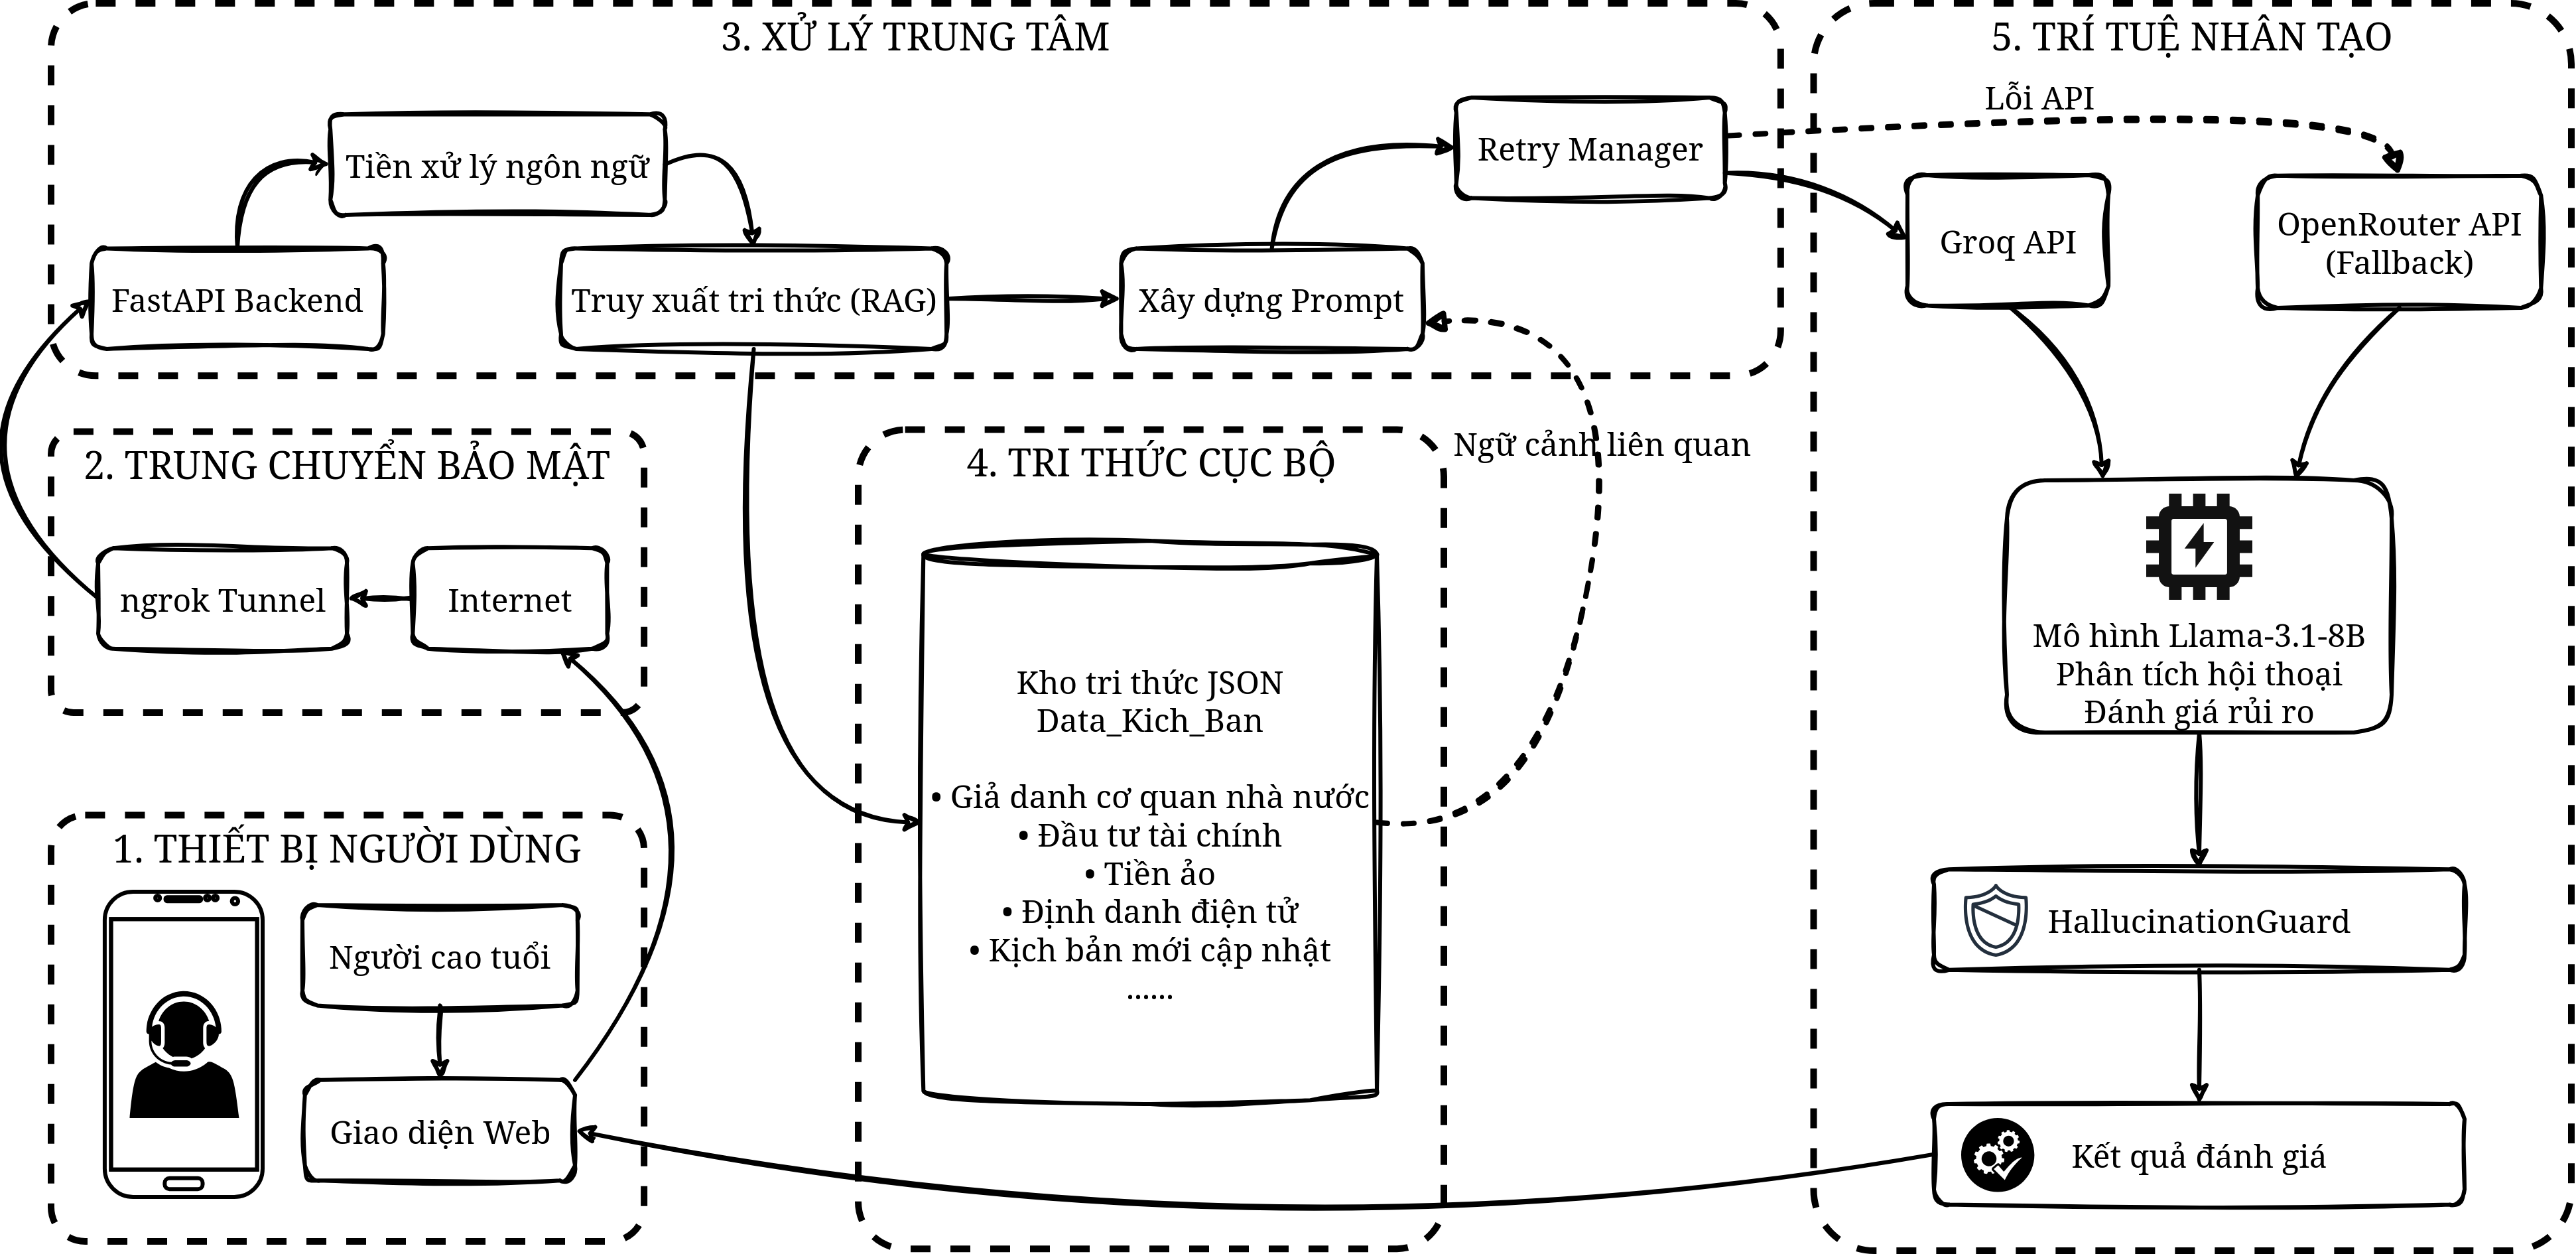
\includegraphics[width=1\linewidth]{kien-truc.png}
    \caption{Kiến trúc hệ thống đề xuất}
    \label{fig:kientruc}
\end{figure}

\section{Luồng hoạt động của hệ thống}
Quá trình xử lý một yêu cầu từ người dùng gồm 12 bước như sau.
\begin{itemize}
    \item Bước 1: Người dùng nhập nội dung cuộc gọi trên giao diện Web, dữ liệu được gửi đến hệ thống dưới dạng JSON.

    \item Bước 2: Render (môi trường demo) tiếp nhận yêu cầu và chuyển tiếp đến FastAPI Backend.

    \item Bước 3: Backend phát hiện và điều chỉnh xưng hô dựa vào đầu vào, sử dụng bảng ánh xạ 33 đại từ nhân xưng (XUNG\_HO\_MAP) và bảy mẫu phát hiện. Ví dụ, nếu người dùng tự xưng "cháu" và gọi hệ thống là "cô", phản hồi dùng cặp "cô/cháu". Nếu người dùng nói "Con ơi", hệ thống nhận ra người lớn tuổi và dùng "con/..." (reverse lookup).

    \item Bước 4: DialectNormalizer chuẩn hóa phương ngữ qua từ điển hơn 110 mục (DIALECT\_MAP), ánh xạ từ địa phương miền Trung và miền Nam sang phổ thông (ví dụ: "mô" $\rightarrow$ "đâu", "răng" $\rightarrow$ "sao", "hổng" $\rightarrow$ "không"). Từ viết hoa ở giữa câu được giữ nguyên để tránh làm thay đổi tên riêng ("Chi" không thành "gì"). Từ viết hoa ở đầu câu vẫn được chuẩn hóa nhưng giữ nguyên chữ hoa đầu.

    \item Bước 5: Backend xác định vùng miền (Bắc, Trung, Nam) dựa trên dấu hiệu từ vựng, dùng ranh giới từ để tránh khớp nhầm (ví dụ "hông" trong "không"). Thông tin vùng miền và dạng chuẩn hóa đầu tiên của câu hỏi được lưu làm "neo" cho các truy vấn RAG ở lượt sau, tránh trôi ngữ cảnh.

    \item Bước 6: Backend quét thư mục Data\_Kich\_Ban, đọc các tệp JSON tri thức. Mỗi khối dữ liệu được tính điểm dựa trên số từ khóa xuất hiện trong câu hỏi. Từ khóa nhiều từ (ví dụ: "chuyển khoản", "mã OTP") được kiểm tra dưới dạng chuỗi con thay vì so khớp rời rạc từng từ. Nếu có từ hai từ khóa trở lên khớp, khối được đưa vào ngữ cảnh; nếu không đủ điểm, khối bị bỏ qua.

    \item Bước 7: Ngữ cảnh RAG được ghép với System Prompt và nội dung hội thoại hiện tại. Hệ thống áp dụng hai chế độ:
    \begin{itemize}
        \item Lượt 1: Dùng ngữ cảnh RAG, System Prompt đầy đủ với cấu trúc ba dòng (chào + nhận dạng / giải thích / lời khuyên).
        \item Lượt 2+: Chuyển sang hội thoại tự do, không dùng RAG, không lặp lại lời chào hay cấu trúc cứng nhắc.
    \end{itemize}

    \item Bước 8: Gọi API Groq với cơ chế thử lại (tối đa hai lần, chờ 1s và 2s). Nếu thất bại, chuyển sang OpenRouter. Nếu cả hai đều lỗi, trả về mã 503 kèm thông báo hệ thống tạm thời không khả dụng.

    \item Bước 9: HallucinationGuard kiểm tra phản hồi: trích xuất các khẳng định, tính điểm neo (grounding score) dựa trên mức độ khớp với ngữ cảnh RAG và nội dung hội thoại, đồng thời phát hiện các mẫu không an toàn. Nếu điểm dưới ngưỡng, phản hồi được thay bằng thông báo thận trọng hơn.

    \item Bước 10: Hệ thống định dạng lại phản hồi thành ba dòng: dòng 1 -- lời chào và nhận dạng rủi ro, dòng 2 -- giải thích, dòng 3 -- lời khuyên. Ở các lượt sau, nếu người dùng gửi "cảm ơn" hoặc "hiểu rồi" mà không kèm câu hỏi, hệ thống phát hiện ý định kết thúc và trả lời chào tạm biệt ngắn gọn.

    \item Bước 11: Backend đóng gói kết quả thành JSON gồm văn bản phản hồi, xưng hô đã phát hiện, vùng miền, số lượt hội thoại và gửi về giao diện Web.

    \item Bước 12: Giao diện hiển thị phản hồi dưới dạng văn bản tự nhiên. Dù trình bày tự do, phản hồi vẫn tuân theo cấu trúc logic: nhận định rủi ro, giải thích lý do dựa trên dấu hiệu phát hiện được, và lời khuyên hành động. Cấu trúc này được đảm bảo qua System Prompt và hậu xử lý.
\end{itemize}

Quy trình xử lý dữ liệu qua các bước được minh họa trong Hình~\ref{fig:luong_xu_ly}.

\begin{figure}[H]
    \centering
    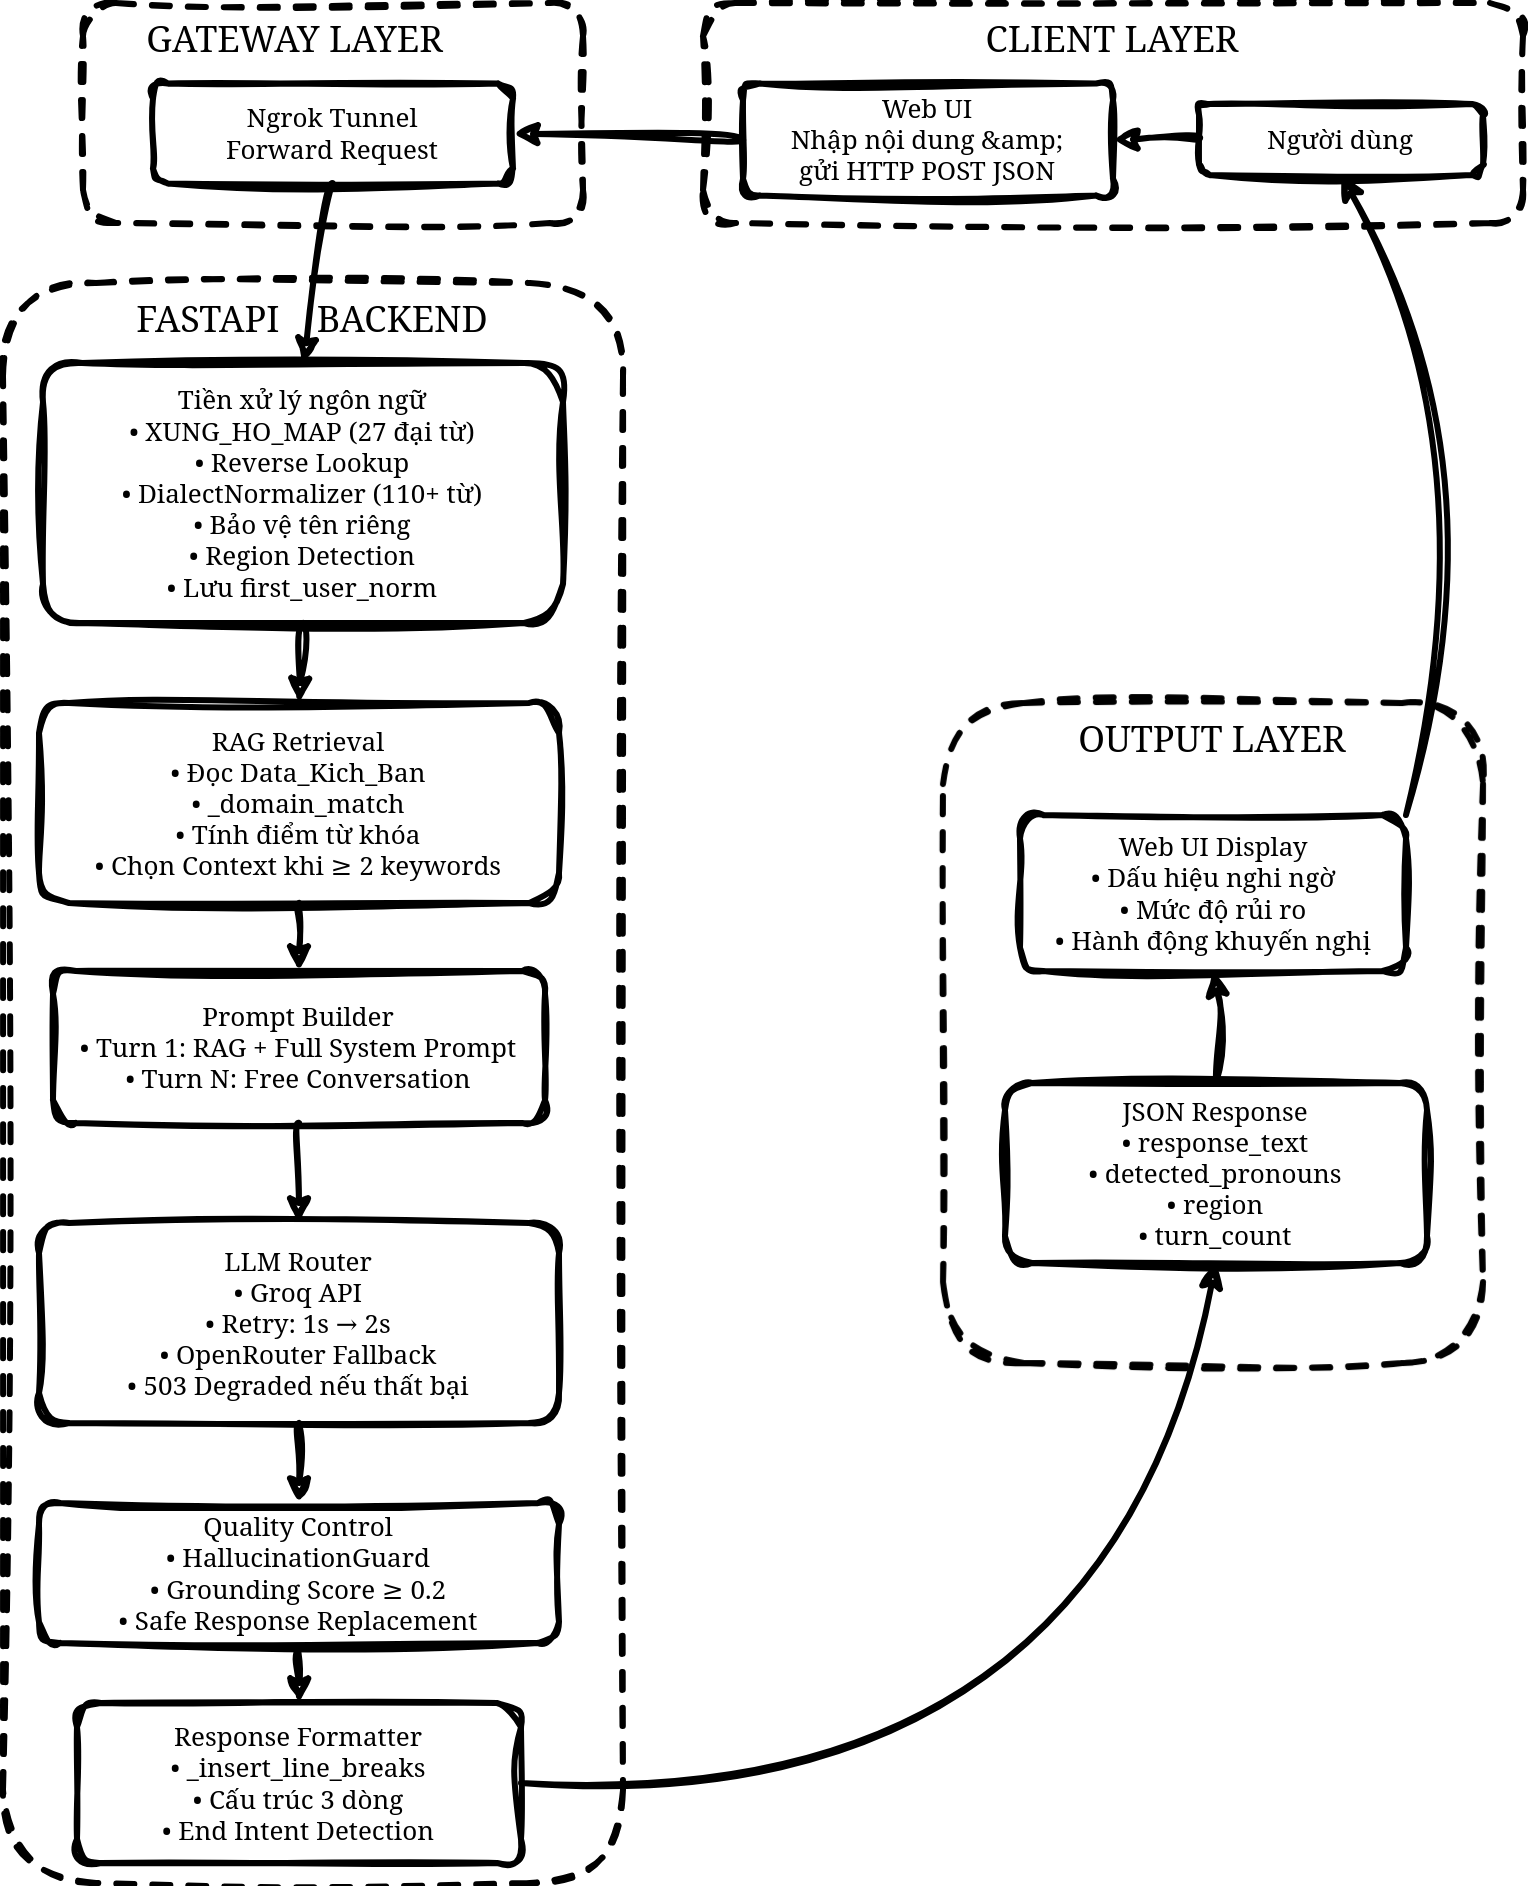
\includegraphics[width=1\linewidth]{luong-xu-li.png}
    \caption{Luồng xử lý của dữ liệu}
    \label{fig:luong_xu_ly}
\end{figure}


%%%%%%%%%%%%%%%%%%%%%%%%%%%%%%%%%%%%%%%%%%%%%%%%%%%
\chapter{KẾT LUẬN}
Sự phát triển mạnh mẽ của công nghệ trong những năm gần đây đã mang lại nhiều lợi ích cho xã hội, đồng thời cũng tạo điều kiện cho các hình thức lừa đảo qua điện thoại ngày càng trở nên tinh vi và khó nhận biết hơn. Trong bối cảnh đó, người cao tuổi là một trong những nhóm đối tượng dễ bị tổn thương nhất do hạn chế về kỹ năng số, khả năng tiếp cận công nghệ và kinh nghiệm nhận diện các mối đe dọa trên môi trường số. Điều này đặt ra nhu cầu cấp thiết về việc xây dựng các công cụ hỗ trợ thông minh nhằm giúp người cao tuổi nâng cao khả năng tự bảo vệ trước các hành vi lừa đảo.

Từ thực tiễn trên, đề tài đã phát triển mô hình chatbot phát hiện lừa đảo điện thoại cho người cao tuổi và tiếp cận bài toán dưới góc độ Trustworthy AI nhằm đảm bảo hệ thống được phát triển theo hướng an toàn, minh bạch và có trách nhiệm đối với người sử dụng.
Đề tài đã phân tích đặc điểm của các hình thức lừa đảo điện thoại phổ biến, đồng thời xây dựng kiến trúc chatbot kết hợp giữa mô hình LLM, cơ sở tri thức (Knowledge Base) và tầng hậu kiểm HallucinationGuard. Cách tiếp cận này cho phép tận dụng khả năng hiểu ngôn ngữ tự nhiên của các mô hình AI hiện đại thông qua Groq Cloud API (Llama-3.1-8B-Instant), trong khi vẫn duy trì khả năng kiểm soát và xác thực kết quả nhằm hạn chế các rủi ro liên quan đến hallucination. Hệ thống cũng triển khai cơ chế dự phòng qua OpenRouter API và xử lý định dạng phản hồi bằng mã nguồn thay vì chỉ dựa vào hướng dẫn ban đầu.

Bên cạnh đó, đề tài đã xây dựng khung phân tích và đánh giá hệ thống dựa trên sáu trục cốt lõi của Trustworthy AI gồm Reliability, Fairness, Robustness, Explainability, Privacy và Social Impact. Đối với từng trục, các thách thức tiềm ẩn đã được phân tích một cách hệ thống, từ nguy cơ hallucination, thiên vị dữ liệu, tấn công Prompt Injection, thiếu minh bạch trong giải thích quyết định cho đến các vấn đề liên quan đến quyền riêng tư và tác động xã hội đối với nhóm người dùng yếu thế. Trên cơ sở đó, các giải pháp thiết kế phù hợp đã được đề xuất nhằm giảm thiểu rủi ro và nâng cao tính đáng tin cậy của hệ thống.

Kết quả phân tích cho thấy rằng việc phát triển một chatbot chống lừa đảo hiệu quả cho người cao tuổi không chỉ là bài toán về độ chính xác của mô hình AI mà còn là bài toán về đạo đức, trách nhiệm và sự chấp nhận của xã hội đối với công nghệ. Một hệ thống chỉ tập trung tối ưu hiệu năng kỹ thuật nhưng bỏ qua các yếu tố công bằng, minh bạch hoặc quyền riêng tư có thể tạo ra những tác động tiêu cực ngoài mong muốn. Ngược lại, việc tích hợp các nguyên tắc của Trustworthy AI ngay từ giai đoạn thiết kế giúp hệ thống trở nên an toàn hơn, dễ được chấp nhận hơn và phù hợp hơn với nhu cầu thực tế của người cao tuổi.

Mặc dù đã đạt được các mục tiêu đề ra, đề tài vẫn còn một số hạn chế. Về hạ tầng, hệ thống phụ thuộc vào Groq Cloud API với giới hạn 500.000 token/ngày, gây khó khăn cho việc kiểm thử quy mô lớn; giải pháp dự phòng OpenRouter vẫn yêu cầu kết nối Internet ổn định. Cơ sở tri thức hiện được lưu dưới dạng tệp JSON tĩnh, chưa hỗ trợ cập nhật động hoặc tích hợp nguồn cảnh báo thời gian thực, đồng thời lỗi chính tả và ký tự đặc biệt trong đầu vào vẫn có thể ảnh hưởng đến chất lượng truy xuất và suy luận. Ngoài ra, khả năng phòng thủ trước tấn công Prompt Injection còn hạn chế: hệ thống mới chỉ áp dụng cơ chế bảo vệ dựa trên hướng dẫn (instruction-based) trong prompt, chưa có tầng lọc đầu vào độc lập bằng regex, chưa tích hợp mô hình phân loại phụ trợ để phát hiện tấn công, và chưa xử lý đầu vào dưới dạng cấu trúc dữ liệu chuẩn để ngăn chặn chỉ thị độc hại lọt vào ngữ cảnh suy luận.

Về khả năng giải thích, hệ thống chưa hỗ trợ lưu vết quyết định lâu dài; log tạm thời của HallucinationGuard bị mất khi khởi động lại. Điểm tin cậy chưa được hiển thị cho người dùng, trong khi grounding score chỉ phục vụ mục đích gỡ lỗi. Khi phát hiện hallucination, hệ thống chỉ trả về thông báo chung mà chưa giải thích rõ nguyên nhân. Các dấu hiệu lừa đảo chưa có cấu trúc dữ liệu chuẩn và cũng chưa tích hợp cơ chế phản hồi từ người dùng để cải thiện mô hình.

Ngoài ra, chức năng chuyển văn bản thành giọng nói TTS chưa được triển khai do hạn chế về thời gian và kĩ thuật, dù đây là tính năng quan trọng đối với người cao tuổi có thị lực kém. Bên cạnh đó, sự thay đổi liên tục của các hình thức lừa đảo đòi hỏi hệ thống phải thường xuyên cập nhật dữ liệu và mô hình để duy trì hiệu quả phát hiện trong dài hạn.

Trong tương lai, hệ thống có thể được mở rộng theo nhiều hướng khác nhau như tích hợp nhận dạng giọng nói theo thời gian thực, bổ sung khả năng phát hiện các cuộc gọi sử dụng công nghệ giả mạo giọng nói (voice cloning), hỗ trợ đa ngôn ngữ và đa phương ngữ, đồng thời kết nối với các nguồn dữ liệu cảnh báo từ cơ quan chức năng hoặc nhà mạng. Bên cạnh đó, việc tìm hiểu sâu hơn về các phương pháp Explainable AI và các cơ chế bảo vệ quyền riêng tư tiên tiến sẽ góp phần nâng cao hơn nữa chất lượng và tính ứng dụng của giải pháp.

Tóm lại, đề tài cho thấy tiềm năng của việc ứng dụng trí tuệ nhân tạo trong hỗ trợ phòng chống lừa đảo điện thoại đối với người cao tuổi, đồng thời khẳng định tầm quan trọng của việc phát triển AI theo định hướng Trustworthy AI. Đây không chỉ là yêu cầu kỹ thuật mà còn là điều kiện cần thiết để các hệ thống trí tuệ nhân tạo có thể được triển khai một cách an toàn, hiệu quả và bền vững trong xã hội số hiện nay.


% \clearpage
% \newpage
% \vspace{0.5cm}
%%%%%%%%%%%%%%%%%%%%%%%%%%%%%%%%%%%%%%%%%%%%%%%%%%%


\end{justify}
\end{spacing}

\printbibliography

\end{document}
